\documentclass[11pt]{article}

\usepackage{graphicx}
\usepackage{mathtools}
\usepackage{amssymb}
\usepackage{titlesec}
\usepackage{hyperref}
\usepackage{varioref}
%\usepackage{tocbibind}
\usepackage{listings}
\usepackage{mathrsfs}
\usepackage{algorithm}
\usepackage{algpseudocode}
\usepackage[a4paper, total={6in, 9.5in}, footnotesep=2\baselineskip]{geometry}
\usepackage[font=small,labelfont=bf,skip=2pt]{caption}
\usepackage[toc,page]{appendix}
\usepackage{enumitem}
\usepackage{array}
\usepackage{multirow}
\usepackage{float}
\usepackage{placeins}
\usepackage{color}
\usepackage{graphics}
\usepackage[utf8]{inputenc}
\usepackage{mdframed}
%\usepackage[Bjornstrup]{fncychap}

\usepackage{csquotes}
\setlength{\parindent}{0em}
\setlength{\parskip}{1em}

\usepackage{listings}
\usepackage{subfigure}

\begin{document}

\begin{titlepage}

\vspace*{\fill}

\newcommand{\HRule}{\rule{\linewidth}{0.5mm}} % Defines a new command for the horizontal lines, change thickness here

\center % Center everything on the page
 
%----------------------------------------------------------------------------------------
%	HEADING SECTIONS
%----------------------------------------------------------------------------------------

\textsc{\LARGE Universitat Politècnica de Catalunya}\\[0.5cm] % Name of your university/college
\textsc{\LARGE Universitat de Barcelona}\\[0.5cm] % Name of your university/college
\textsc{\LARGE Universitat Rovira i Virgili}\\[1.5cm] % Name of your university/college
\textsc{\Large Master in Artificial Intelligence}\\[0.5cm] % Major heading such as course name
\textsc{\large Planning and Approximate Reasoning}\\[0.5cm] % Minor heading such as course title

%----------------------------------------------------------------------------------------
%	TITLE SECTION
%----------------------------------------------------------------------------------------

\HRule \\[0.4cm]
{ \huge \bfseries The Coffee Problem}\\[0.4cm] % Title of your document
\HRule \\[1.5cm]
 
%----------------------------------------------------------------------------------------
%	AUTHOR SECTION
%----------------------------------------------------------------------------------------

%\begin{minipage}{0.4\textwidth}
%\begin{flushleft} \large
%\emph{Author:}\\
%Alejandro \textsc{Su\'arez Hern\'andez} \\
%\end{flushleft}
%\end{minipage}
%~
%\begin{minipage}{0.4\textwidth}
%\begin{flushright} \large
%\emph{Director:} \\
%Carme \textsc{Torras Gen\'is} \\
%\emph{Co-director:}\\
%Guillem \textsc{Aleny\`a Ribas} \\
%\emph{Tutor:}\\
%Javier \textsc{B\'ejar Alonso} % Supervisor's Name
%\end{flushright}
%\end{minipage}\\[4cm]

% If you don't want a supervisor, uncomment the two lines below and remove the section above
\Large \emph{Authors:}\\
Emanuel \textsc{Sanchez Aimar}\\ % Your name
Johannes \textsc{Heidecke}\\[3cm] % Your name

%----------------------------------------------------------------------------------------
%	DATE SECTION
%----------------------------------------------------------------------------------------

{\large November 2016}\\[3cm] % Date, change the \today to a set date if you want to be precise

%----------------------------------------------------------------------------------------
%	LOGO SECTION
%----------------------------------------------------------------------------------------

%\includegraphics{Logo}\\[1cm] % Include a department/university logo - this will require the graphicx package
 
%----------------------------------------------------------------------------------------

\vspace*{\fill} % Fill the rest of the page with whitespace

\end{titlepage}


\tableofcontents
\listoffigures
\lstlistoflistings

\clearpage

\chapter{Fuzzy Variables}

\section{Input Variables}

There are four input variables used in this fuzzy system that describe relevant features of each player of the game. The variables \texttt{daysPerWeek} and \texttt{minutesPerDay} describe the players commitment to the game measured in time units. The variables \texttt{currentLevel} and \texttt{currentPoint} describe the players progress in the game. The linguistic labels for each variable, as well as their value range and membership functions are described and justified in the following subsections. 

\subsection{daysPerWeek}

The \texttt{daysPerWeek} variable describes the activeness of the user measured in days per week on a scale from 0 to 7 with three linguistic labels: 'occasionally', 'regularly' and 'fully'. The respective membership functions are trapezoidal, their parameters can be seen in table \ref{tab:daysPerWeek}:

\begin{table}[H]
\centering
\begin{tabular}{@{}lll@{}}
\toprule
\textbf{linguistic label}  & \textbf{trapezoidal function} \\ 
\midrule
occasionally  & $(0,0,2,3)$ \\
regularly & $(2,3,5,6)$ \\
fully & $(5,6,7,7)$ \\
\bottomrule
\end{tabular}
\caption{Linguistic labels for \texttt{daysPerWeek}}
\label{tab:daysPerWeek}
\end{table}

As we can see graphically in figure \ref{fig:daysPerWeek}, the membership functions are not balanced. The labels 'occasionally' and 'regularly' take up more of the possible values than 'fully'.

\begin{figure}[H]
\centering
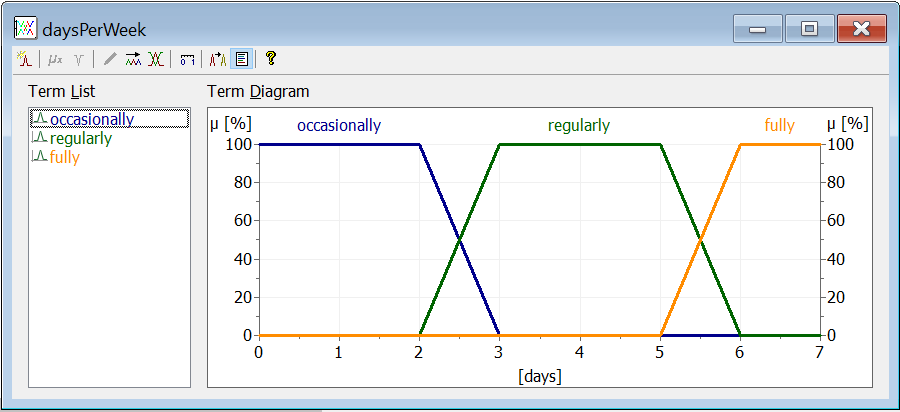
\includegraphics[width=\textwidth]{img/vDaysPerWeek}
\caption{Membership functions of \texttt{daysPerWeek} variable}
\label{fig:daysPerWeek} 
\end{figure}

\subsection{minutesPerDay}

The \texttt{minutesPerDay} variable describes the activeness of the user, measured in minutes per day on a scale from 0 to 180 with four linguistic labels: 'negligible', 'short', 'right',  and 'large'. The respective membership functions are trapezoidal, their parameters can be seen in table \ref{tab:minutesPerDay}:

\begin{table}[H]
\centering
\begin{tabular}{@{}lll@{}}
\toprule
\textbf{linguistic label}  & \textbf{trapezoidal function} \\ 
\midrule
negligible  & $(0,0,5,15)$ \\
short & $(5,15,25,30)$ \\
right & $(25,30,60,90)$ \\
large & $(60,90,180,180)$ \\
\bottomrule
\end{tabular}
\caption{Linguistic labels for \texttt{minutesPerDay}}
\label{tab:minutesPerDay}
\end{table}

As we can see graphically in figure \ref{fig:minutesPerDay}, the membership functions are not balanced. The labels 'negligible' and 'short' have a relatively small value range, while 'large' alone covers more than half of the possible values.

\begin{figure}[H]
\centering
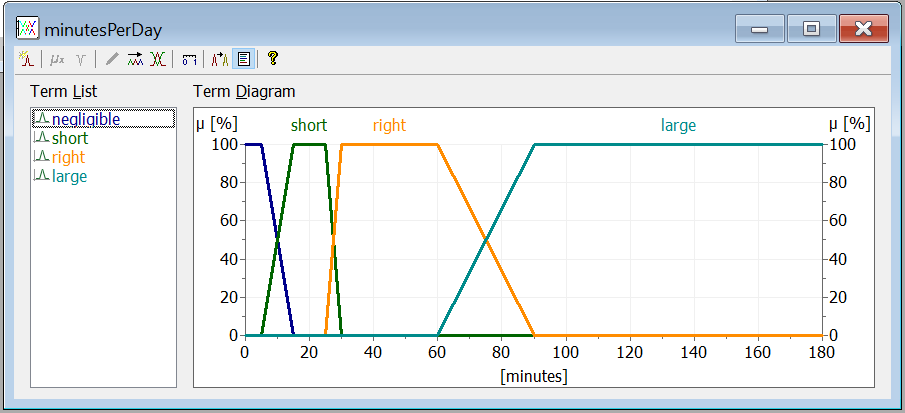
\includegraphics[width=\textwidth]{img/vMinutesPerDay}
\caption{Membership functions of \texttt{minutesPerDay} variable}
\label{fig:minutesPerDay} 
\end{figure}

\subsection{currentLevel}

The input varialbe \texttt{currentLevel} describes the progress of the user in the game measured with his current level. Its values range from 1 (start level) to 60 (maximum level). There are three linguistic labels to describe a player: 'beginner' for new players who do not have a lot of experience, 'intermediate' for players with some experience who still haven't proceeded to the late stage of the game, and 'advanced' for players who are close to finishing the game. The membership functions of these labels can be seen in table \ref{tab:currentLevel}.

\begin{table}[H]
\centering
\begin{tabular}{@{}lll@{}}
\toprule
\textbf{linguistic label}  & \textbf{trapezoidal function} \\ 
\midrule
beginner  & $(0,0,10,20)$ \\
intermediate & $(10,20,40,50)$ \\
advanced & $(40,50,60,60)$ \\
\bottomrule
\end{tabular}
\caption{Linguistic labels for \texttt{currentLevel}}
\label{tab:currentLevel}
\end{table}

The labels of \texttt{currentLevel} are unbalanced. The range of levels for which players are considered to be 'intermediate' is wider than for both 'beginner' and 'advanced'. This reflects the notion that players surmount the 'beginner' stadium rather quickly but then need a relatively long time to proceed towards being 'advanced'. This can be observed graphically in the plot of membership functions in figure \ref{fig:currentLevel}.

\begin{figure}[H]
\centering
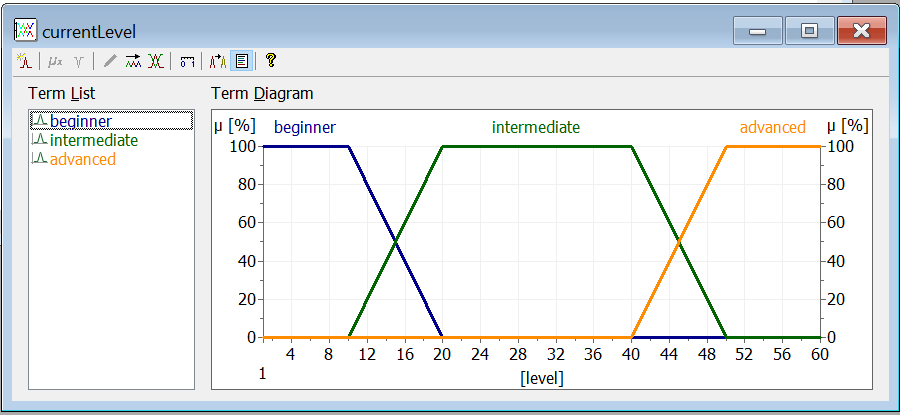
\includegraphics[width=\textwidth]{img/vCurrentLevel}
\caption{Membership functions of \texttt{currentLevel} variable}
\label{fig:currentLevel} 
\end{figure}

\subsection{currentPoints}

The variable \texttt{currentPoints} describes the amount of points of a player with the four linguistic labels 'few', 'some', 'average', and 'many'. A player can have between 0 and 1000 points and based on the current number of points and the membership functions of the labels, it gets assigned certain degrees of membership to the labels. The parameters of the trapezoidal membership functions are summarized in table \ref{tab:currentPoints}.

\begin{table}[H]
\centering
\begin{tabular}{@{}lll@{}}
\toprule
\textbf{linguistic label}  & \textbf{trapezoidal function} \\ 
\midrule
few  & $(0,0,100,150)$ \\
some & $(100,150,400,500)$ \\
average & $(400,500,700,800)$ \\
many & $(700,800,1000,1000)$ \\
\bottomrule
\end{tabular}
\caption{Linguistic labels for \texttt{currentPoints}}
\label{tab:currentPoints}
\end{table}

The unbalanced labels reflect the subjective judgement when saying 'few' or 'some': \textit{``a few points''} is a more narrow concept that \textit{``some points''}. This can be seen in the plotted membership functions in figure \ref{fig:currentPoints}. 

\begin{figure}[H]
\centering
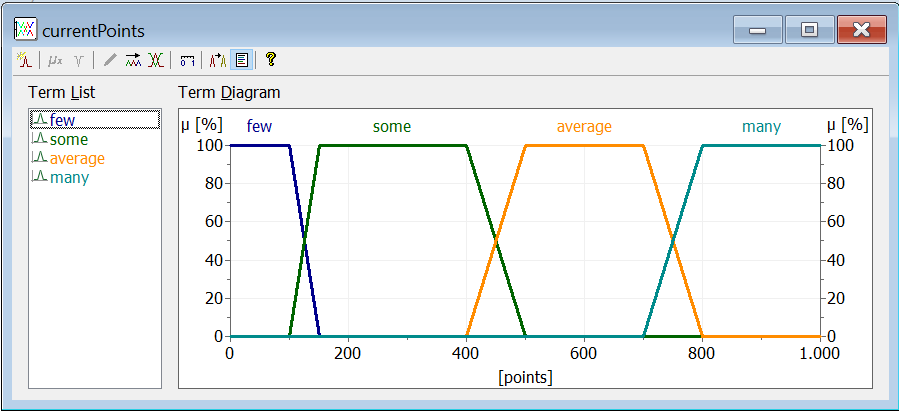
\includegraphics[width=\textwidth]{img/vCurrentPoints}
\caption{Membership functions of \texttt{currentPoints} variable}
\label{fig:currentPoints} 
\end{figure}

\section{Output Variables}

The system has two output variables: \texttt{addictionDegree} and \texttt{waitingMinutes}. The former describes the degree to which a player is addicted to the game. The latter defines how long a user needs to wait after loosing his lives in the game until he can start playing again. The more committed a player is to the game and the more advanced he is, the longer he should be asked to wait in order to increase the probabilities of them spending money on shortening the waiting time. Thus, the \texttt{addictionDegree} variable is both an output variable and an input variable to determine the best value for \texttt{waitingMinutes}. A more detailed overview of the connections between the variables and rule blocks is given in chapter \ref{cha:rb}.

\subsection{addictionDegree}

The output variable \texttt{addictionDegree} defines a players level of addiction to the game. The values range from 0 to 100 and are covered by three labels: 'lazy', 'normal' and 'eager'. The membership functions for these labels are trapezoidal and their parameters can be seen in table \ref{tab:addictionDegree}.

\begin{table}[H]
\centering
\begin{tabular}{@{}lll@{}}
\toprule
\textbf{linguistic label}  & \textbf{trapezoidal function} \\ 
\midrule
lazy  & $(0,0,15,25)$ \\
normal & $(15,25,75,85)$ \\
eager & $(75,85,100,100)$ \\
\bottomrule
\end{tabular}
\caption{Linguistic labels for \texttt{addictionDegree}}
\label{tab:addictionDegree}
\end{table}

The labels are unbalanced - players are considered to have a 'normal' addiction degree for a larger range of values than being considered 'lazy' or 'eager'. This corresponds to the subjective human understanding of addiction degree. The membership functions are plotted in figure \ref{fig:addictionDegree}.

\begin{figure}[H]
\centering
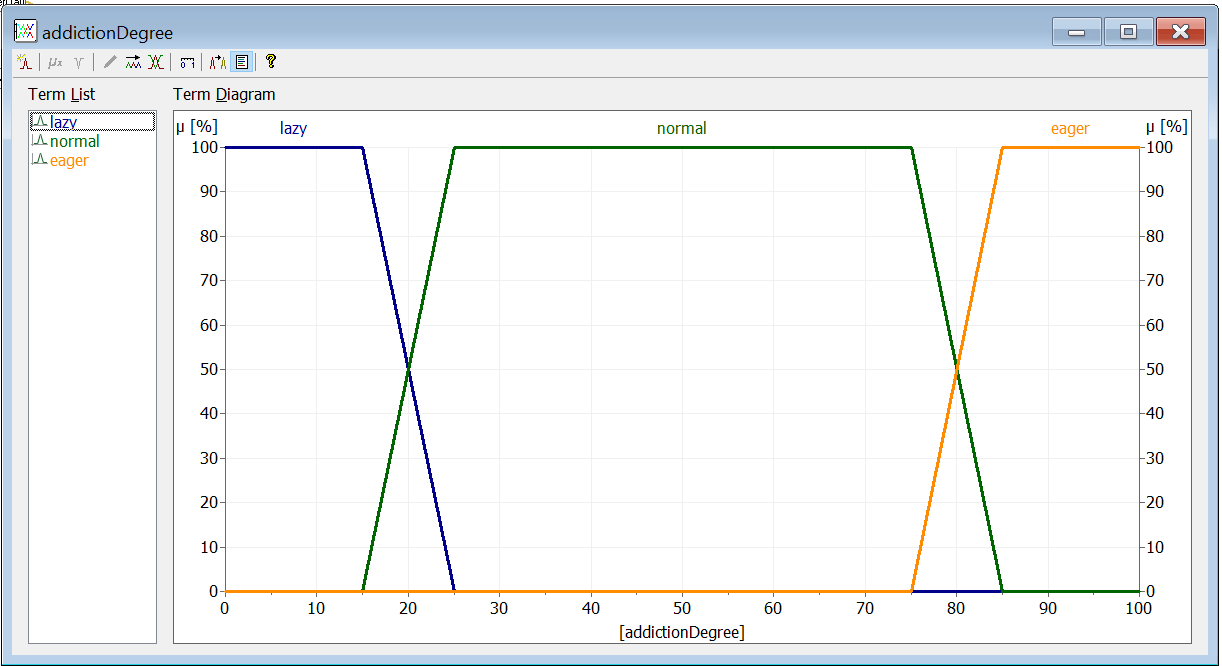
\includegraphics[width=\textwidth]{img/vAddictionDegree}
\caption{Membership functions of \texttt{addictionDegree} variable}
\label{fig:addictionDegree} 
\end{figure}

\subsection{waitingMinutes}

The variable \texttt{waitingMinutes} outputs how long a player needs to wait after loosing their in-game lives. If a player needs to wait too long it might lead to them abandoning the game. On the other hand, if the waiting time is too short to begin with, they will not spend money on making it shorter. The waiting time is always within a range between 0 and 120 minutes and is divided into five linguistic labels: 'veryShort', 'short', 'medium', 'long', and 'almostForever'. Their corresponding trapezoidal membership functions are depicted in table \ref{tab:waitingMinutes}.

\begin{table}[H]
\centering
\begin{tabular}{@{}lll@{}}
\toprule
\textbf{linguistic label}  & \textbf{trapezoidal function} \\ 
\midrule
veryShort  & $(0,0,5,10)$ \\
short & $(5,10,20,30)$ \\
medium & $(20,30,45,60)$ \\
long & $(45,60,90,105)$ \\
almostForever & $(90,105,120,120)$ \\
\bottomrule
\end{tabular}
\caption{Linguistic labels for \texttt{waitingMinutes}}
\label{tab:waitingMinutes}
\end{table}

The labels of \texttt{waitingMinutes} are distributed in an unbalanced way. The notion of 'veryShort', for example, lies on a much narrower value range than that of 'long'. This can be observed in the plotted membership functions of figure \ref{fig:waitingMinutes}.

\begin{figure}[H]
\centering
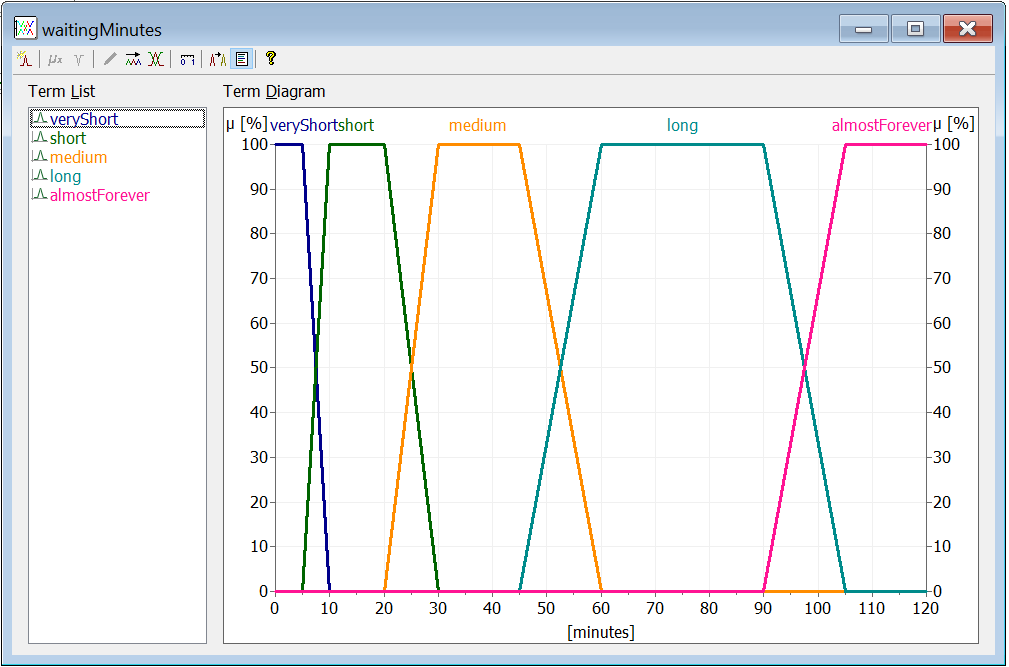
\includegraphics[width=\textwidth]{img/vWaitingMinutes}
\caption{Membership functions of \texttt{waitingMinutes} variable}
\label{fig:waitingMinutes} 
\end{figure}

\chapter{Rule Blocks}
\label{cha:rb}

The variables described in the previous section are connected by two rule blocks. The first rule block, described in section \ref{sec:rb1}, combines the input variables \texttt{minutesPerDay} and \texttt{daysPerWeek} to output a value of \texttt{addictionDegree}. The second rule block, described in section \ref{sec:rb2}, combines the output of the first rule block and the input variables \texttt{currentLevel} and \texttt{currentPoints} to output a value of \texttt{waitingMinutes}. The structure of the fuzzy system is shown in figure \ref{fig:all}.

\begin{figure}[H]
\centering
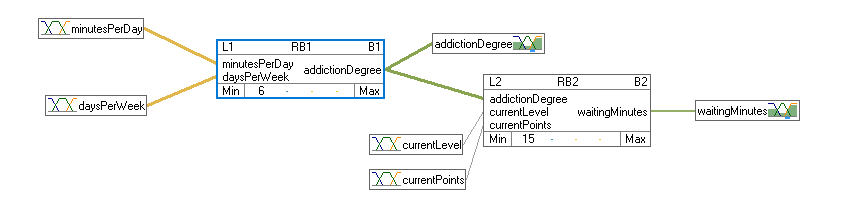
\includegraphics[width=\textwidth]{img/all}
\caption{Overview of variables and rule blocks}
\label{fig:all} 
\end{figure}

\section{Rules for addictionDegree}
\label{sec:rb1}

There are six fuzzy rules that combine the labels of \texttt{minutesPerDay} and \texttt{daysPerWeek} to deduce a label of \texttt{addictionDegree}. The first rule, \texttt{R1}, covers all cases in which the player plays only a 'negligible' amount of minutes per day: in these cases the \texttt{addictionDegree} is 'lazy'. The same deduction is done in \texttt{R2} for all players with the label \texttt{daysPerWeek.occasionally}. There are also conjunctive rules, such as \texttt{R4} in which a player is labelled as 'eager' if he has both the label \texttt{minutesPerDay.right} and \texttt{daysPerWeek.fully}. This rule block covers all possible combinations of the two input variables. Since the two input variables are probably highly correlated, in many cases one variable provides enough information about the player's addiction level. For example, if we know that a player plays only 'occasionally', the addiction degree will not be higher than 'lazy'. All rules can be seen in figure \ref{fig:rb1}.

\begin{figure}[H]
\centering
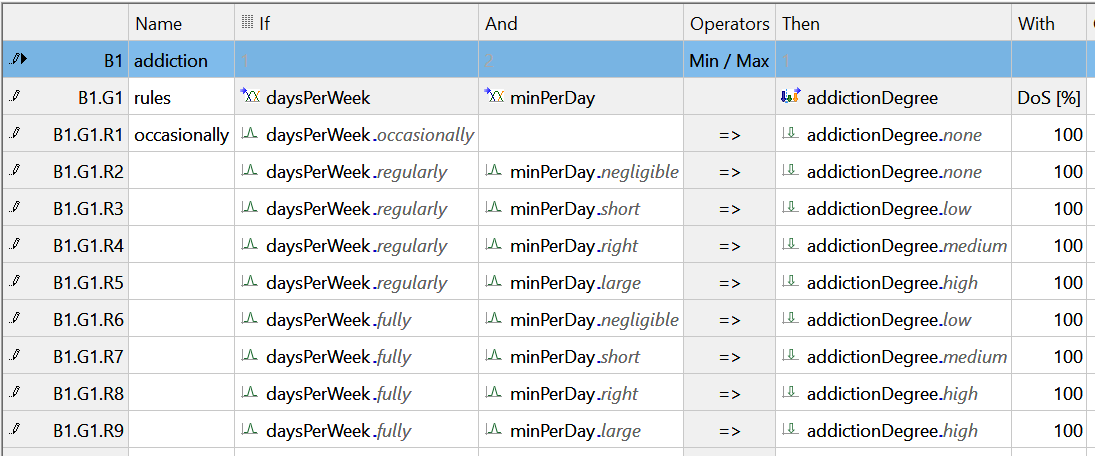
\includegraphics[width=\textwidth]{img/rb1}
\caption{Rule block for addictionDegree}
\label{fig:rb1} 
\end{figure}

\section{Rules for waitingMinutes}
\label{sec:rb2}

The second rule block is larger and more complex - it combines three input variables (one of them being the output of rule block 1 and the other ones being \texttt{currentLevel} and \texttt{currentPoints}) to the \texttt{waitingMinutes} output variable. Generally, the \texttt{waitingMinutes} increase with higher addictionDegree of the player, since a high addiction makes the player willing to wait longer or even motivates him to spend money on the game. A higher level also correlates with a longer wait time - the player has potentially invested many resources into the game and is incentivized to stay longer. Similarly, a high number of points increases the waiting time and thus motivates the player to spend these points. There are 15 different rules in the rule block, all covering at least a conjunction of 2 input variables. All possible cases are covered by the rules, with some cases slightly overlapping. The specific rules are depicted in figure \ref{fig:rb2}.

\begin{figure}[H]
\centering
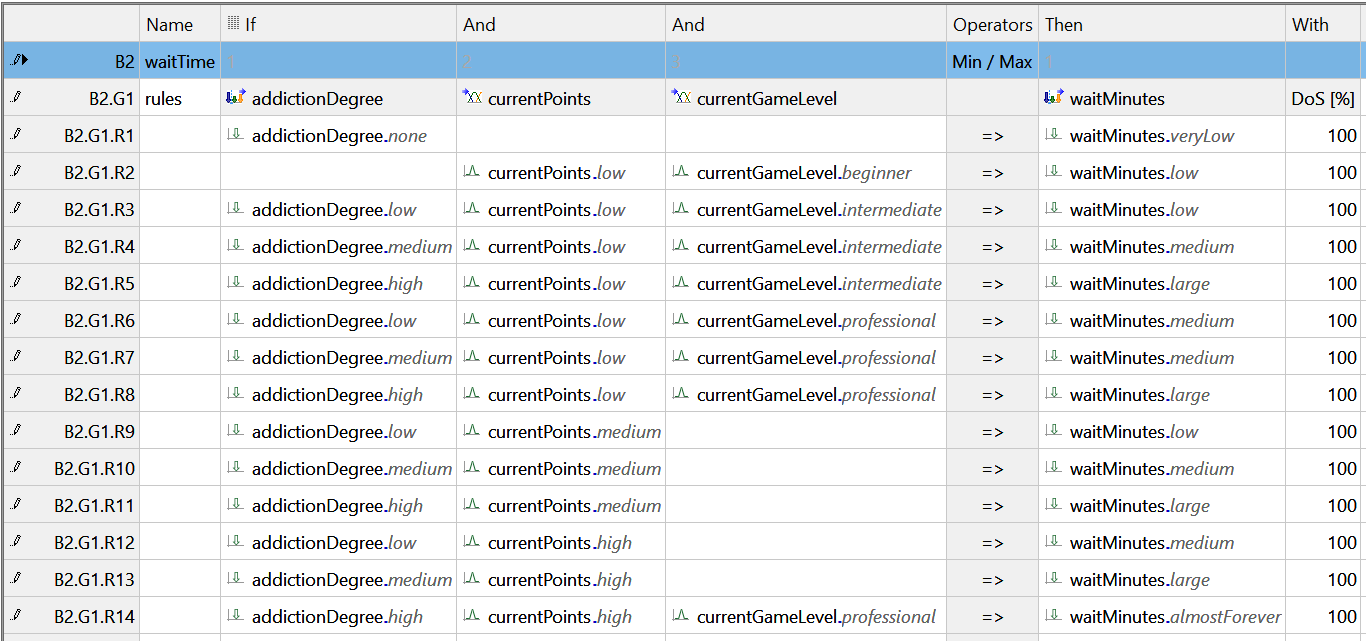
\includegraphics[width=\textwidth]{img/rb2}
\caption{Rule block for waitingMinutes}
\label{fig:rb2} 
\end{figure}

\chapter{Results}

\section{Manual calculation}

\subsection{User profile}

For the manual calculations based on the variables and rule blocks defined in the previous sections, a user profile was chosen that activates several labels and rules at the same time and is therefore interesting to observe. The chosen input variables are as summarized in table 

\begin{table}[H]
\centering
\begin{tabular}{@{}lll@{}}
\toprule
\textbf{variable}  & \textbf{input value} \\ 
\midrule
\texttt{minutesPerDay} & 83 \\
\texttt{daysPerWeek}  & 5.4 \\
\texttt{currentLevel} & 42 \\
\texttt{currentPoints} & 420 \\
\bottomrule
\end{tabular}
\caption{System input for manual calculations}
\label{tab:prof0}
\end{table}

\subsection{Fuzzyfication}
\label{sub:fuzzyfic}

The value $83$ for \texttt{minutesPerDay} lies between the labels 'right' $(25,30,60,90)$ and 'large' $(60,90,180,190)$.

\[ right: \frac{90-83}{90-60} \cdot 100\% = 23.\overline{3}\% \]
\[ large: \frac{83-60}{90-60} \cdot 100\% = 76.\overline{6}\% \]
\vspace{1em}

The value $5.4$ for \texttt{daysPerWeek} lies between the labels 'regularly' $(2,3,5,6)$ and 'fully' $(5,6,7,7)$.

\[ regularly: \frac{6-5.4}{6-5} \cdot 100\% = 60\% \]
\[ fully: \frac{5.4-5}{6-5} \cdot 100\% = 40\% \]
\vspace{1em}

The value $42$ for \texttt{currentLevel} lies between the labels 'intermediate' $(10,20,40,50)$ and 'advanced' $(40,50,60,60)$.

\[ intermediate: \frac{50-42}{50-40} \cdot 100\% = 80\% \]
\[ advanced: \frac{42-40}{50-40} \cdot 100\% = 20\% \]
\vspace{1em}

The value $420$ for \texttt{currentPoints} lies between the labels 'some' $(100,150,400,500)$ and 'average' $(400,500,700,800$).

\[ some: \frac{500-420}{500-400} \cdot 100\% = 80\% \]
\[ many: \frac{420-400}{500-400} \cdot 100\% = 20\% \]
\vspace{1em}

\subsection{Activation of addictionDegree}

The output variable \texttt{addictionDegree} depends on both \texttt{minutesPerDay} and \texttt{daysPerWeek}. From the previous section we know the activation of the labels for these two input variables: $23.\overline{3}\%$ for \texttt{minutesPerDay.right}, $76.\overline{6}\%$ for \texttt{large}, $60\%$ for \texttt{daysPerWeek.regularly}, and $40\%$ for \texttt{daysPerWeek.fully}. Looking at the rules in the relevant rule block (see section \ref{sec:rb1}) we can see that the following rules are activated:
\[ R4: right \wedge regularly \Rightarrow normal \]
\[ R5: right \wedge fully \Rightarrow eager \]
\[ R6: large \Rightarrow eager \]

Using the minimum operator for conjunctions, we obtain:

\[ R4: 23.\overline{3}\% \Rightarrow normal \]
\[ R5: 23.\overline{3}\% \Rightarrow eager \]
\[ R6: 76.\overline{6}\% \Rightarrow eager \]

Since we have several rules activating for the output label 'eager', we apply the maximum operator and obtain:

\[ 23.\overline{3}\% \Rightarrow normal \]
\[ 76.\overline{6}\% \Rightarrow eager \]

\subsection{Defuzzyfication of addictionDegree}

% --- normal:

To get the activated area of the 'normal' label we calculate the trapezoid of the label's membership function $(15,25,75,85)$ under the activation line $\mu = 23.\overline{3}$. The x-value of the intercept with the trapezoid and $\mu = 23.\overline{3}$ between $15$ and $25$ is:

\[ \frac{x_1-15}{25-15} \cdot 100\% = 23.\overline{3} \Leftrightarrow x_1 = 2.\overline{3} + 15 \Leftrightarrow x_1 = 17.\overline{3} \]

Equivalently, the intercept of the 'normal' trapezoid and $\mu = 23.\overline{3}$ between $75$ and $85$ is:

\[ \frac{85-x_2}{85-75} \cdot 100\% = 23.\overline{3} \Leftrightarrow x_2 = 85 - 2.\overline{3} \Leftrightarrow x_2 = 82.\overline{6} \]

Thus, the corner points of the resulting activated trapezoid are: 
\[A_{normal} = \{(15,0),(17.\overline{3},23.\overline{3}),(82.\overline{6},23.\overline{3}),(85,0) \}\]


% --- eager:

To get the activated area of the 'eager' label we calculate the trapezoid of the label's membership function $(75,85,100,100)$ under the activation line $\mu = 76.\overline{6}$. The x-value of the intercept with the trapezoid and $\mu = 76.\overline{6}$ between $75$ and $80$ is:

\[ \frac{x_1-75}{85-75} \cdot 100\% = 76.\overline{6} \Leftrightarrow x_1 =  82.\overline{6} \]

The resulting corner points of the activated trapezoid are:

\[A_{eager} = \{(75,0), (82.\overline{6},76.\overline{6}), (100,76.\overline{6}), (100,0) \}\]

We now have to take the maximum of the activated areas $A_{normal}$ and $A_{eager}$ for each $x$-value. $A_{normal}$ is obviously larger than $A_{eager}$ for $ x < 75 $. Thus, we have to find the intercept between  $A_{normal}$ and $A_{eager}$ in the range $ x \in [75, 82.\overline{6}]$ to determine the point $x^*$ at which $A_{eager}$ has higher $\mu$ values than $A_{normal}$ for $x > x^*$. We intercept the lines $\mu = 23.\overline{3}$ (coming from $A_{normal}$) and the line between $(75,0)$ and  $(82.\overline{6},76.\overline{6})$:

\[ \frac{x^*-75}{82.\overline{6}-75} \cdot 76.\overline{6}\% = 23.\overline{3} \Leftrightarrow x^* = 77.\overline{3} \]

With this information we know all corner points of the activated area for the \texttt{addictionDegree} variable:

\[ A_{addictionDegree} = \{ (15,0),(17.\overline{3},23.\overline{3}), (77.\overline{3},23.\overline{3}), (82.\overline{6},76.\overline{6}), (100,76.\overline{6}), (100,0)  \}\]

For defuzzyfication we use the \textit{Center of Area} (CoA) approach and try to find an $\overline{x}$ for which the activated area is the same on both sides.

To do this we first calculate the total area. We split up the shape into triangles and rectangles to calculate the area geometrically:

\[ A_{x \in [15,17.\overline{3}]} = \frac{1}{2} \cdot (17.\overline{3} - 15) \cdot (23.\overline{3} - 0 ) = 27.\overline{2} \]
\[ A_{x \in [17.\overline{3},77.\overline{3}]} = (77.\overline{3} - 17.\overline{3}) \cdot  (23.\overline{3} - 0 ) = 1400 \]
\[ A_{x \in [77.\overline{3},82.\overline{6}]} = (82.\overline{6} - 77.\overline{3}) \cdot ((23.\overline{3} - 0) + \frac{1}{2} \cdot (76.\overline{6} - (23.\overline{3})) = 266.\overline{6} \]
\[ A_{x \in [82.\overline{6},100]} = (100-82.\overline{6}) \cdot (76.\overline{6}-0) = 1328.\overline{8} \]

Summing up, we get to a total area of:

\[ A_{x \in [15,100]} = A_{x \in [15,17.\overline{3}]} + A_{x \in [17.\overline{3},77.\overline{3}]} + A_{x \in [77.\overline{3},82.\overline{6}]} + A_{x \in [82.\overline{6},100]} = 3022.\overline{6} \]

Thus, we are looking for $\overline{x}$ with 
\[ A_{x \in [15,\overline{x}]} = 3022.\overline{6} \cdot \frac{1}{2} = 1511.\overline{3} \]

We know that $A_{x \in [15,17.\overline{3}]} + A_{x \in [17.\overline{3},77.\overline{3}]} = 1427.\overline{2} $. Hence, we can reformulate the problem to find:

\[ A_{x \in [77.\overline{3},\overline{x}]} = 1511.\overline{3} - 1427.\overline{2} = 84.\overline{1} \]

Since $ A_{x \in [77.\overline{3},82.\overline{6}]} = 266.\overline{6} $ and $266.\overline{6} > 84.\overline{1}$ , we can search for a solution in the interval $[77.\overline{3},82.\overline{6}]$. The linear function that describes the top border of the area's segment between $[77.\overline{3},82.\overline{6}]$ can be described for $z = x -77.\overline{3}, x \in [77.\overline{3},82.\overline{6}] $ as

\[ f(z) = 23.\overline{3} + \frac{76.\overline{6} -23.\overline{3} }{82.\overline{6}-77.\overline{3}} \cdot z = 23.\overline{3} + 10z\]

We want to find $\overline{z}$ for which the integral of $f$ from 0 to $\overline{z}$ equals $84.\overline{1}$:

\[ \int_0^{\overline{z}} f(z) = 84.\overline{1} \Leftrightarrow [23.\overline{3}z + 5z^2]_0^{\overline{z}} = 84.\overline{1} \]

\[ \Rightarrow [23.\overline{3}\overline{z} + 5\overline{z}^2] - [0] = 84.\overline{1}\]

\[ \Rightarrow - 84.\overline{1} + 23.\overline{3}\overline{z} + 5\overline{z}^2  = 0\]

\[ \Rightarrow z_1 = 2.385, z_2 = -7.05 \]

Since $z$ can't be negative, we know that $\overline{z} = 2.385 $ and thus $\overline{x} = 2.385 + 77.\overline{3} $. We found the Center of Areas to be at an addiction degree of $79.7183$.

\subsection{Activation of waitingMinutes}

The output variable \texttt{waitingMinutes} depends on the two input variables \texttt{currentLevel} and \texttt{currentPoints}, as well as the output of \texttt{addictionDegree}. From section \ref{sub:fuzzyfic} we know the membership degrees of the labels for the two input variables. In the previous section we obtained the defuzzyfied value of the \texttt{addictionDegree} as $79.7183$. To make the following manual calculations a bit shorter while only slightly changing the final results, we round the \texttt{addictionDegree} up to $80.0$. This gives us an activation of \texttt{addictionDegree.normal} and \texttt{addictionDegree.eager} of exactly $50\%$ each. The activated rules of the rule block (see section \ref{sec:rb2}) are:

\[ R9: normal \wedge intermediate \wedge some \Rightarrow medium \]
\[ R10: normal \wedge advanced  \wedge some \Rightarrow long \]
\[ R13: eager \wedge intermediate \Rightarrow long \]
\[ R14: advanced \wedge many \Rightarrow almostForever \]
\[ R15: eager \wedge advanced \Rightarrow almostForever \]

Using the minimum operator for conjunctions, we obtain:

\[ R9: 20\% \Rightarrow medium \]
\[ R10: 20\% \Rightarrow long \]
\[ R13: 50\% \Rightarrow long \]
\[ R14: 20\% \Rightarrow almostForever \]
\[ R15: 20\% \Rightarrow almostForever \]

Since we have several rules activating for the output labels 'long' and 'almostForever', we apply the maximum operator and obtain:

\[ 20\% \Rightarrow medium \]
\[ 50\% \Rightarrow long \]
\[ 20\% \Rightarrow almostForever \]

\subsection{Defuzzyfication of waitingMinutes}

% --- medium:

To get the activated area of the 'medium' label we calculate the trapezoid of the label's membership function $(20,30,45,60)$ under the activation line $\mu = 20$. The x-value of the intercept with the trapezoid and $\mu = 20$ between $20$ and $30$ is:

\[ \frac{x_1-20}{30-20} \cdot 100\% = 20 \Leftrightarrow x_1 = 22 \]

Equivalently, the intercept of the 'medium' trapezoid and $\mu = 20$ between $45$ and $60$ is:

\[ \frac{60-x_2}{60-45} \cdot 100\% = 20 \Leftrightarrow x_2 = 57 \]

Thus, the corner points of the resulting activated trapezoid are: 
\[A_{medium} = \{ (20,0), (22,20), (57,20), (60,0) \}\]

% --- long:

To get the activated area of the 'long' label we calculate the trapezoid of the label's membership function $(45,60,90,105)$ under the activation line $\mu = 50$. The x-value of the intercept with the trapezoid and $\mu = 50$ between $45$ and $60$ is:

\[ \frac{x_1-45}{60-45} \cdot 100\% = 50 \Leftrightarrow x_1 = 52.5 \]

Equivalently, the intercept of the 'long' trapezoid and $\mu = 50$ between $90$ and $105$ is:

\[ \frac{105-x_2}{105-90} \cdot 100\% = 50 \Leftrightarrow x_2 = 97.5 \]

Thus, the corner points of the resulting activated trapezoid are: 
\[A_{long} = \{ (45,0), (52.5,50), (97.5,50), (105,0) \}\]


% --- almostForever:

To get the activated area of the 'almostForever' label we calculate the trapezoid of the label's membership function $(90,105,120,120)$ under the activation line $\mu = 20$. The x-value of the intercept with the trapezoid and $\mu = 20$ between $90$ and $105$ is:

\[ \frac{x_1-90}{105-90} \cdot 100\% = 20 \Leftrightarrow x_1 = 93 \]

Thus, the corner points of the resulting activated trapezoid are: 
\[A_{almostForever} = \{ (90,0),(93,20),(120,20),(120,0) \}\]


% --- total area:
We now have to take the maximum of the activated areas $A_{medium}$, $A_{long}$, and $A_{almostForever}$ for each $x$-value. $A_{medium}$ is  larger than $A_{long}$ for $ x < 45 $. Thus, we have to find the intercept between  $A_{medium}$ and $A_{long}$ in the range $ x \in [45,52.5]$ to determine the point $x^*$ at which $A_{long}$ has higher $\mu$ values than $A_{medium}$ for $x > x^*$. We intercept the lines $\mu = 20$ (coming from $A_{medium}$) and the line between $(45,0)$ and  $(52.5,50)$:

\[ \frac{x_1^*-45}{52.5-45} \cdot 50\% = 20 \Leftrightarrow x_1^* = 48 \]

$A_{almostForever}$ is  larger than $A_{long}$ for $ x > 105 $. Thus, we have to find the intercept between  $A_{almostForever}$ and $A_{long}$ in the range $ x \in [97.5,105]$ to determine the point $x^*$ at which $A_{long}$ has higher $\mu$ values than $A_{almostForever}$ for $x < x^*$. We intercept the lines $\mu = 20$ (coming from $A_{almostForever}$) and the line between $(97.5,50)$ and  $(105,0)$:

\[ \frac{105-x_2^*}{105-97.5} \cdot 50\% = 20 \Leftrightarrow x_2^* = 102 \]


With this information we know all corner points of the activated area for the \texttt{waitingMinutes} variable:

\[ A_{waitingMinutes} = \{ (20,0),(22,20),(48,20),(52.5,50),(97.5,50),(102,20),(120,20),(120,0)  \}\]

For defuzzyfication we use the \textit{Center of Area} (CoA) approach and try to find an $\overline{x}$ for which the activated area is the same on both sides.

To do this we first calculate the total area. We split up the shape into triangles and rectangles to calculate the area geometrically:

\[ A_{x \in [20,22]} = \frac{1}{2} \cdot (22-20) \cdot (20-0) = 20 \]
\[ A_{x \in [22,48]} = (48-22) \cdot (20-0) = 520 \]
\[ A_{x \in [48,52.5]} = (52.5-48) \cdot ((20-0) + \frac{1}{2}\cdot(50-20) ) = 157.5 \]
\[ A_{x \in [52.5,97.5]} = (97.5-52.5) \cdot (50-0) = 2250 \]
\[ A_{x \in [97.5,102]} = (102-97.5) \cdot ((20-0) + \frac{1}{2}\cdot(50-20) ) = 157.5 \]
\[ A_{x \in [102,120]} = (120-102) \cdot (20-0) = 360 \]

Summing up all areas we get:

\[ A_{x \in [20,120]} = 3465 \]

Thus, we are looking for $\overline{x}$ with 
\[ A_{x \in [20,120]} = 3465 \cdot \frac{1}{2} = 1732.5 \]

We know that $A_{x \in [20,52.5]}  = 697.5 $. Hence, we can reformulate the problem to find:

\[ A_{x \in [52.5,\overline{x}]} = 1732.5 - 697.5 = 1035 \]

Since the area $A_{x \in [52.5,97.5]}$ is a rectangle, we can obtain $\overline{x}$ with the equation 

\[ \overline{x} = 52.5 + \frac{1035}{2250} * (97.5-52.5) = 73.2 \]

Thus, the defuzzyfied value for \texttt{waitingMinutes} is $73.2$.

\section{Automatic calculation}

For the automatically calculated results, we define three user profiles with different, interesting features that lead to the activation of multiple rules at the same time. The user profiles are described in section \ref{sub:users} and the results of the fuzzy system are presented in section \ref{sub:autoRes}.

\subsection{User profiles}
\label{sub:users}

We define three user profiles reflecting different types of users: the 'enthusiastic beginner' (profile 1), the 'motivated veteran' (profile 2), and the 'skeptical beginner' (profile 3).

The 'enthusiastic beginner' has shortly started the game but is already spending a lot of time on it. His input variables can be seen in table \ref{tab:prof1}.

\begin{table}[H]
\centering
\begin{tabular}{@{}lll@{}}
\toprule
\textbf{variable}  & \textbf{input value} \\ 
\midrule
\texttt{minutesPerDay} & 80 \\
\texttt{daysPerWeek}  & 5.5 \\
\texttt{currentLevel} & 5 \\
\texttt{currentPoints} & 120 \\
\bottomrule
\end{tabular}
\caption{Input variables of profile 1: 'enthusiastic beginner'}
\label{tab:prof1}
\end{table} 

The 'motivated veteran' has played the game for a long time and while he is still an active player, his activity has gone down a bit recently. His input variables can be seen in table \ref{tab:prof2}

\begin{table}[H]
\centering
\begin{tabular}{@{}lll@{}}
\toprule
\textbf{variable}  & \textbf{input value} \\ 
\midrule
\texttt{minutesPerDay} & 28 \\
\texttt{daysPerWeek}  & 4 \\
\texttt{currentLevel} & 55 \\
\texttt{currentPoints} & 740 \\
\bottomrule
\end{tabular}
\caption{Input variables of profile 2: 'motivated veteran'}
\label{tab:prof2}
\end{table}

The 'skeptical beginner' is also fairly new to the game and is not yet convinced to spend a lot of time on playing it. His input variables can be seen in table \ref{tab:prof3}

\begin{table}[H]
\centering
\begin{tabular}{@{}lll@{}}
\toprule
\textbf{variable}  & \textbf{input value} \\ 
\midrule
\texttt{minutesPerDay} & 12 \\
\texttt{daysPerWeek}  & 2.2 \\
\texttt{currentLevel} & 5 \\
\texttt{currentPoints} & 50 \\
\bottomrule
\end{tabular}
\caption{Input variables of profile 3: 'skeptical beginner'}
\label{tab:prof3}
\end{table}

\subsection{Results for output variables}
\label{sub:autoRes}


For the profile 1, 'enthusiastic beginner', figure \ref{fig:p1mpd} shows the activations of the \texttt{minutesPerDay} labels. The player is considered to be mostly active with the 'large' label and to a third also to the 'right' label.

\begin{figure}[H]
\centering
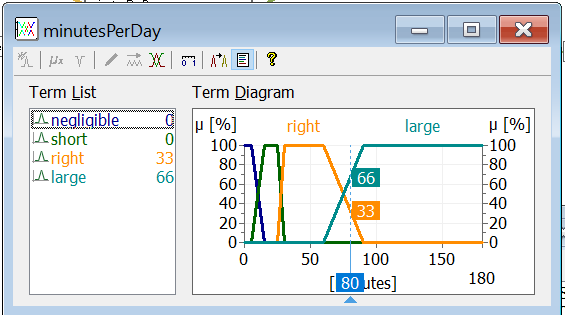
\includegraphics[width=\textwidth]{img/profile1_vMinutesPerDay}
\caption{\texttt{minutesPerDay} for profile 1}
\label{fig:p1mpd} 
\end{figure}

Figure \ref{fig:p1ad} shows the area activated for the \texttt{addictionDegree} and the corresponding defuzzyfied center of areas value of $65.918$. The player's addiction level is still considered to be normal, but towards the upper spectrum of normal.

\begin{figure}[H]
\centering
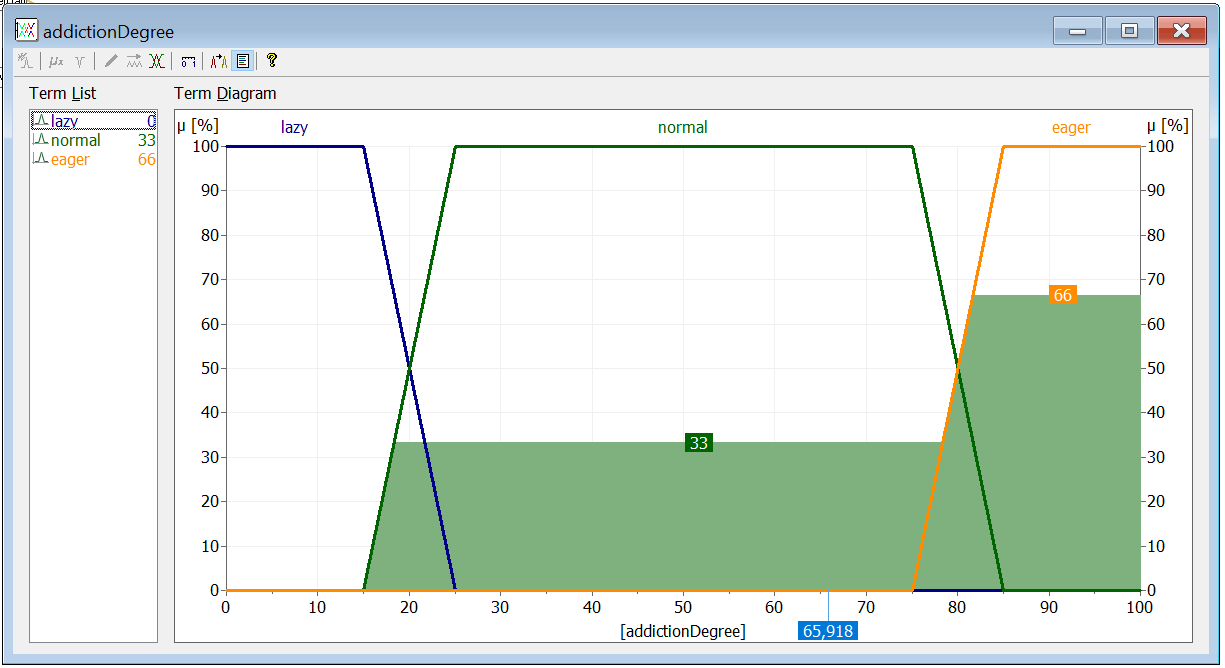
\includegraphics[width=\textwidth]{img/profile1_vAddictionDegree}
\caption{\texttt{addictionDegree} for profile 1}
\label{fig:p1ad} 
\end{figure}

Figure \ref{fig:p1wm} shows the calculated waiting time the system came up with. With $33.51$ minutes the player has to wait for a time that is perceived as lower-medium.

\begin{figure}[H]
\centering
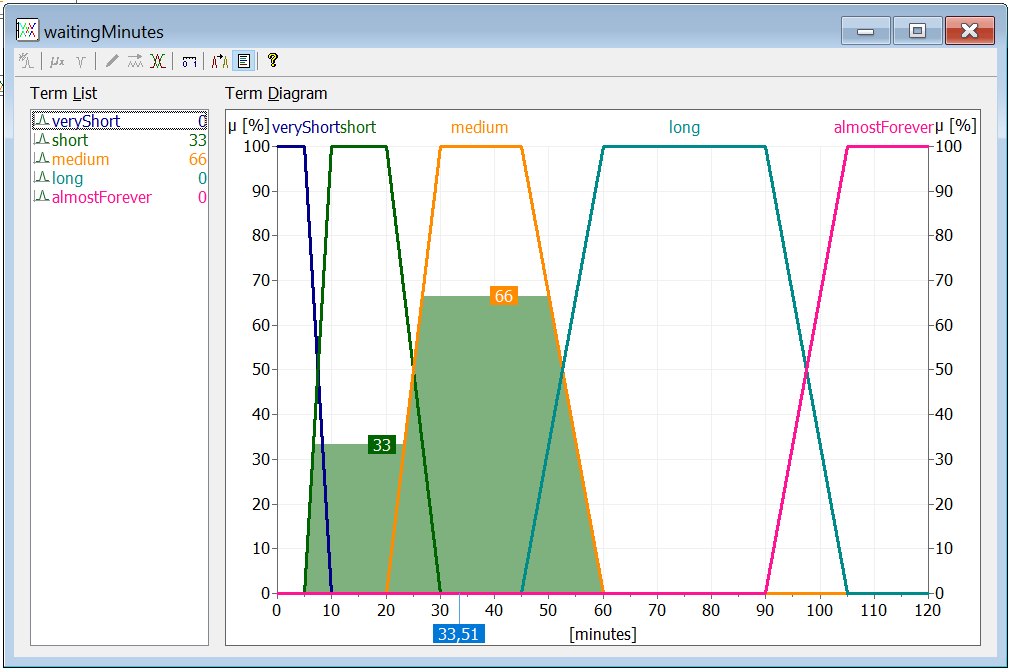
\includegraphics[width=\textwidth]{img/profile1_vWaitingMinutes}
\caption{\texttt{waitingMinutes} for profile 1}
\label{fig:p1wm} 
\end{figure}

Figure \ref{fig:prof1} shows an overivew of all input and output variables for the 'enthusiastic beginner'.

\begin{figure}[H]
\centering
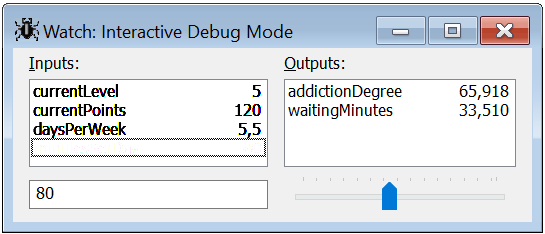
\includegraphics[width=\textwidth]{img/profile1}
\caption{Output variables for profile 1}
\label{fig:prof1} 
\end{figure}

In figure \ref{fig:p2mpd} we show the activations of \texttt{minutesPerDay} for the player with profile 2: 'motivated veteran'. The player is considered to play just a 'right' amount of minutes per day, with a 40\% membership degree to the 'short' label. This shows that the player is still playing enough, but is threatening to become more inactive.

\begin{figure}[H]
\centering
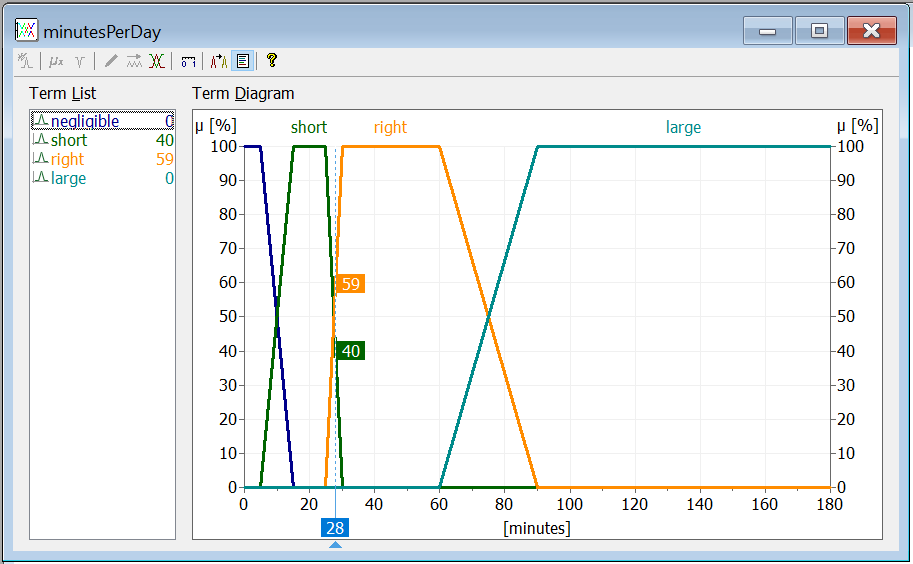
\includegraphics[width=\textwidth]{img/profile2_vMinutesPerDay}
\caption{\texttt{minutesPerDay} for profile 2}
\label{fig:p2mpd} 
\end{figure}

The addiction degree of the second player is perfectly normal as can be seen in figure \ref{fig:p2ad}. All activated rules label the player with having a normal degree of addiction.

\begin{figure}[H]
\centering
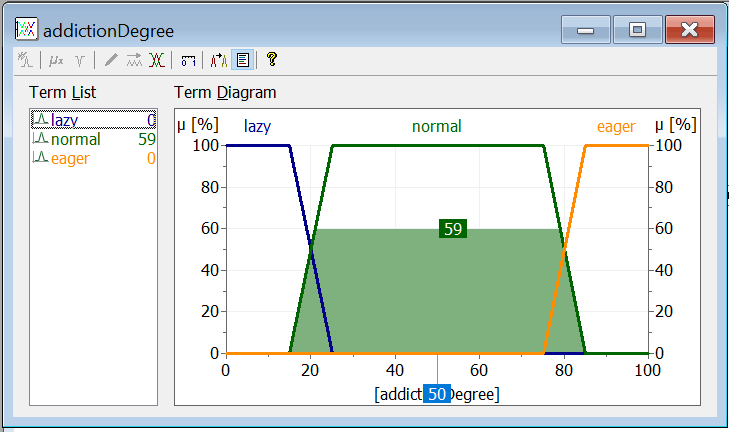
\includegraphics[width=\textwidth]{img/profile2_vAddictionDegree}
\caption{\texttt{addictionDegree} for profile 2}
\label{fig:p2ad} 
\end{figure}

Figure \ref{fig:p2wm} shows that the system assigns a rather high waiting time to the player. His high level and points lead to the system considering a 'almostForever' waiting time, which moves the center of areas to 83.34 minutes.

\begin{figure}[H]
\centering
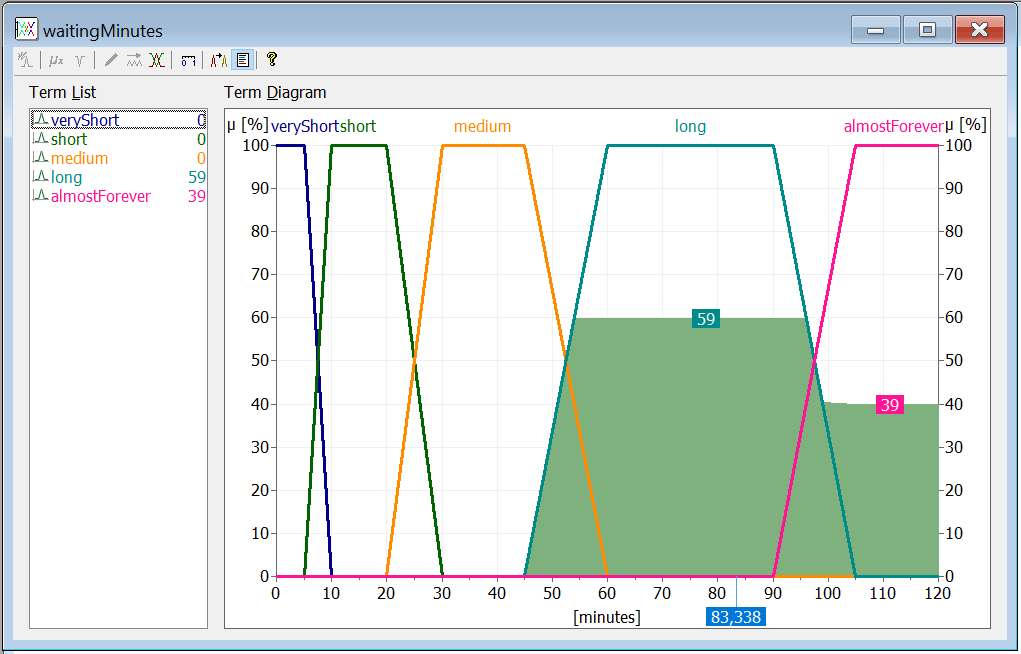
\includegraphics[width=\textwidth]{img/profile2_vWaitingMinutes}
\caption{\texttt{waitingMinutes} for profile 2}
\label{fig:p2wm} 
\end{figure}

In figure \ref{fig:prof2} we see an overview of all input and output variables for the second profile.

\begin{figure}[H]
\centering
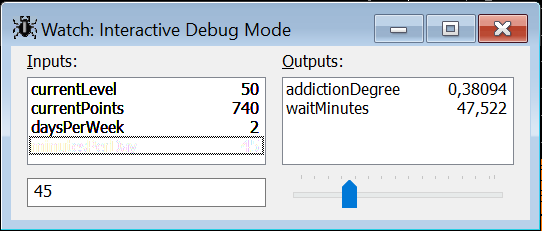
\includegraphics[width=\textwidth]{img/profile2}
\caption{Output variables for profile 2}
\label{fig:prof2} 
\end{figure}

The player of profile 3, 'skeptical beginner', has a daily play time that is considered 'short' with $\mu=70$ and even 'negligible' with $\mu=29$, see figure \ref{fig:p3mpd}.

\begin{figure}[H]
\centering
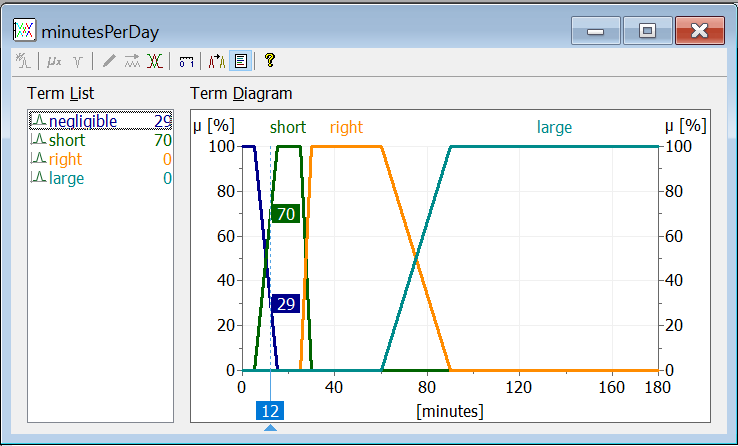
\includegraphics[width=\textwidth]{img/profile3_vMinutesPerDay}
\caption{\texttt{minutesPerDay} for profile 3}
\label{fig:p3mpd} 
\end{figure}

The skeptical attitude of this player towards the game is reflected in his defuzzyfied \texttt{addictionDegree}. As we can see in figure \ref{fig:p3ad}, this players addiction degree is the lowest of all profiles with only $39.024$.

\begin{figure}[H]
\centering
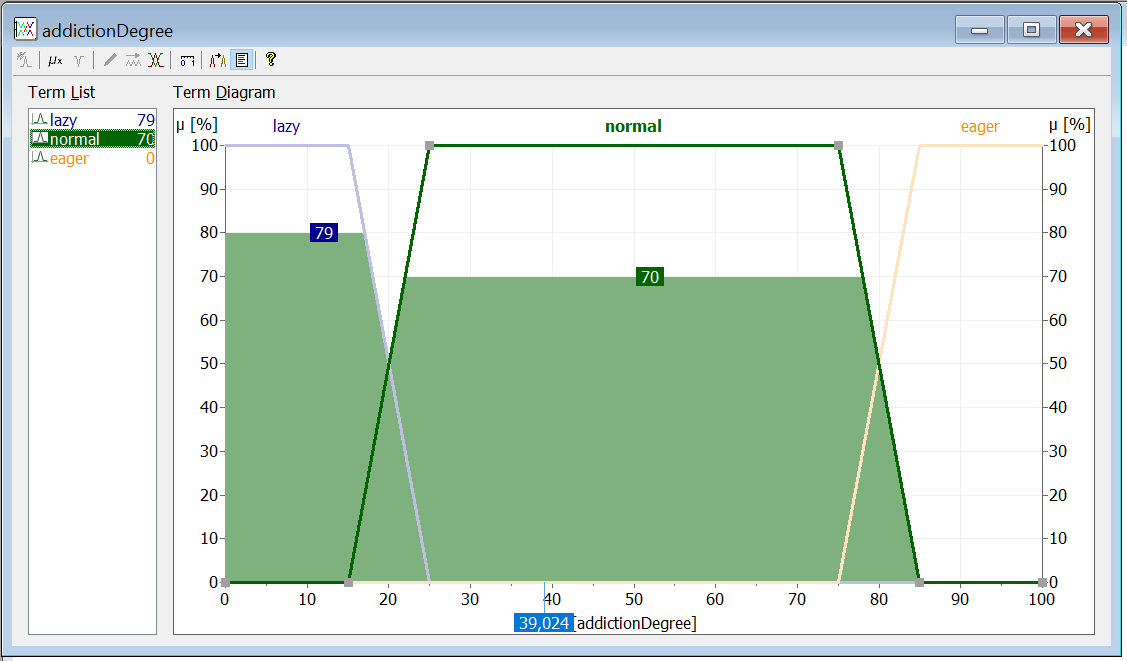
\includegraphics[width=\textwidth]{img/profile3_vAddictionDegree}
\caption{\texttt{addictionDegree} for profile 3}
\label{fig:p3ad} 
\end{figure}

In figure \ref{fig:p3wm} we show the proposed waitingMinutes for this player. With waiting for only about 12 minutes, the player has an incentive to return to the game quickly which will hopefully increase his addiction degree. A higher waiting time might change his mind towards leaving the game.

\begin{figure}[H]
\centering
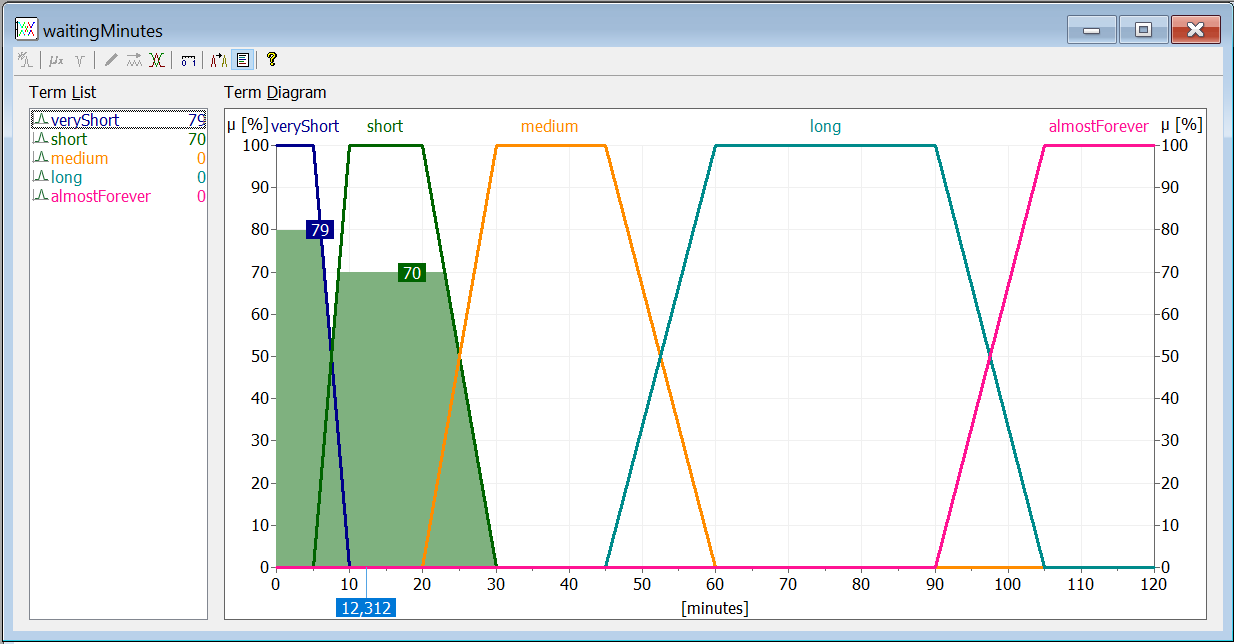
\includegraphics[width=\textwidth]{img/profile3_vWaitingMinutes}
\caption{\texttt{waitingMinutes} for profile 3}
\label{fig:p3wm} 
\end{figure}

An overview of the profile's variables is shown in figure \ref{fig:prof3}.

\begin{figure}[H]
\centering
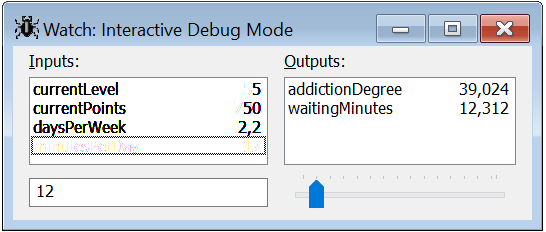
\includegraphics[width=\textwidth]{img/profile3}
\caption{Output variables for profile 3}
\label{fig:prof3} 
\end{figure}

It can be interesting to observe the relationship between multiple variables on an output variable. In figure \ref{fig:prof1_3d} we can see the relationship between \texttt{currentLevel} and \texttt{currentPoints} for a player of profile 1 (with an \texttt{addictionDegree} of 65.918). In general it can be observed, that as planned the rules define a function that increases the waiting time with increasing level and with increasing points. A speciality that can be observed here is that for low levels, the waiting time increases when reaching 400 points or more but then decreases again around 800 points. This is justified by trying to incentivize players with low levels who are accumulating points towards spending the points and not hoarding them. If this incentive does not work (the points keep increasing while the level stays low), the waiting time decreases again to make sure that the player levels up faster and reaches more interesting parts of the game. The highest waiting time is clearly for players who have both a very high level and a high number of points. It can be seen, that the \texttt{currentLevel} variable has generally a higher impact on the waiting time than the \texttt{currentPoints}.


\begin{figure}[H]
\centering
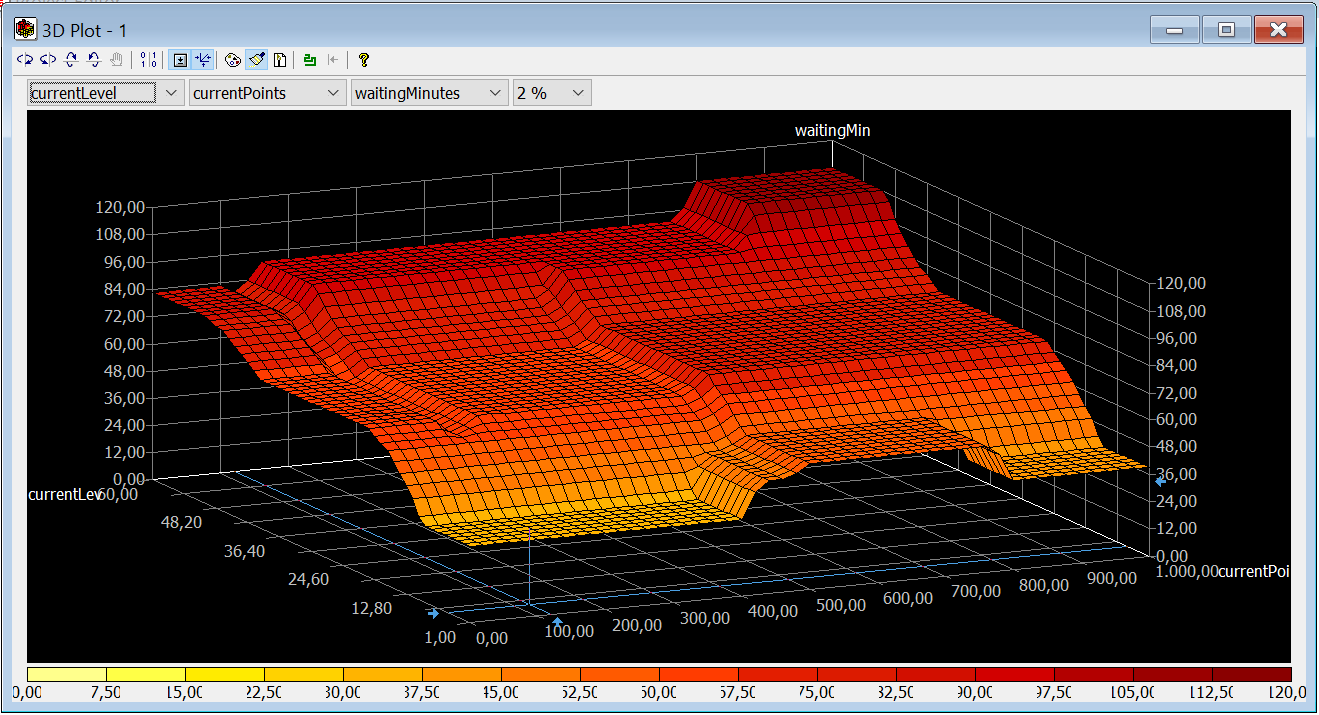
\includegraphics[width=\textwidth]{img/profile1_3d}
\caption{Effect of \texttt{currentLevel} and \texttt{currentPoints} on \texttt{waitingMinutes} for profile 1}
\label{fig:prof1_3d} 
\end{figure}

Each rule in the rule blocks can be assigned with a \textit{degree of support} that changes the impact of the rule on the final results. For example, when changing the degree of support for \texttt{R12} ($eager \wedge beginner \Rightarrow medium $) in the \texttt{waitingTime} rule block for profile 1, there is a clearly observable effect on the calculated waiting time. While for a support of 100\% the waitingTime, the calculated waiting time is 33.5 (figure \ref{fig:prof1_3d100}), it decreases to 30.190 when decreasing the support of the rule to 50\% (figure \ref{fig:prof1_3d50}), and even further to only 21.882 minutes when decreasing the support to 10\% (figure \ref{fig:prof1_3d10}). Decreasing the support of this rule removes the support for letting the player wait a 'medium' duration if the player is 'eager' and a 'beginner'. This decreases the waiting time for the player of profile 1 (who fulfills these criteria) when decreasing the rules degree of support.
 
\begin{figure}[H]
\centering
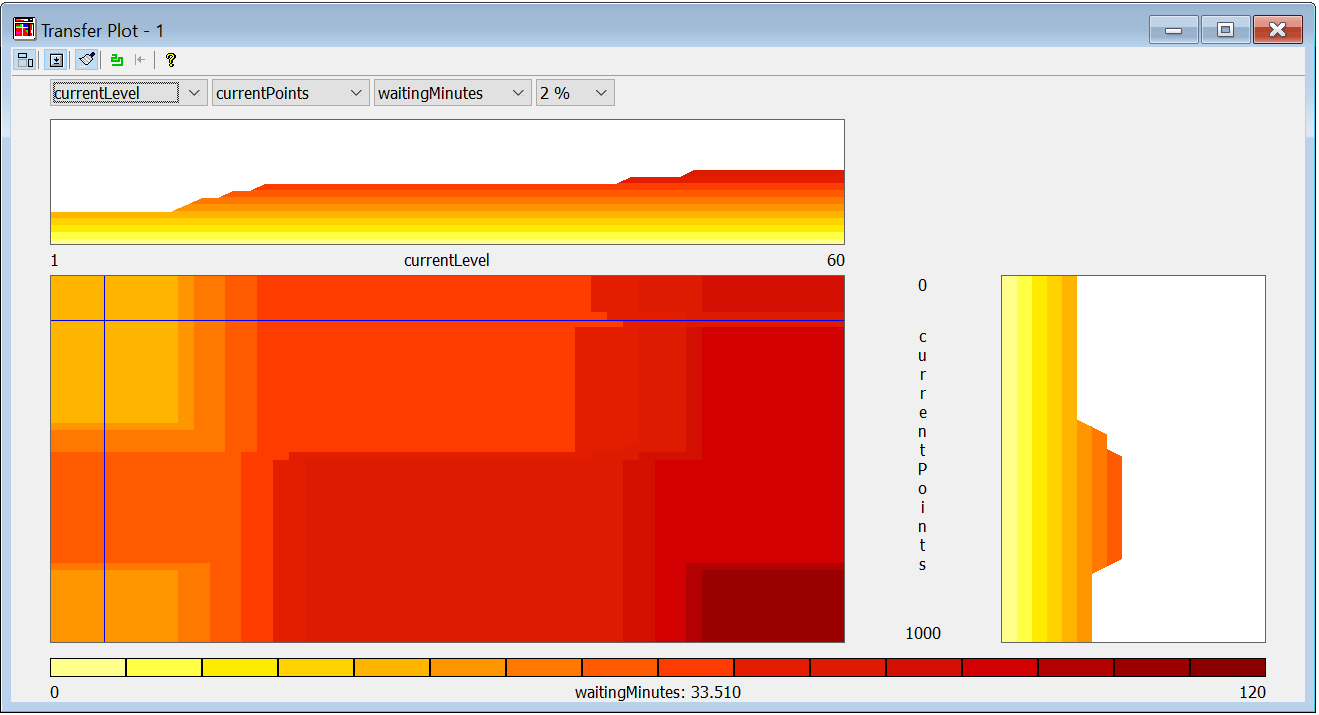
\includegraphics[width=\textwidth]{img/profile1_r12-100}
\caption{Heatmap of \texttt{waitingMinutes} activation for \texttt{R12}=100\%}
\label{fig:prof1_3d100} 
\end{figure}

\begin{figure}[H]
\centering
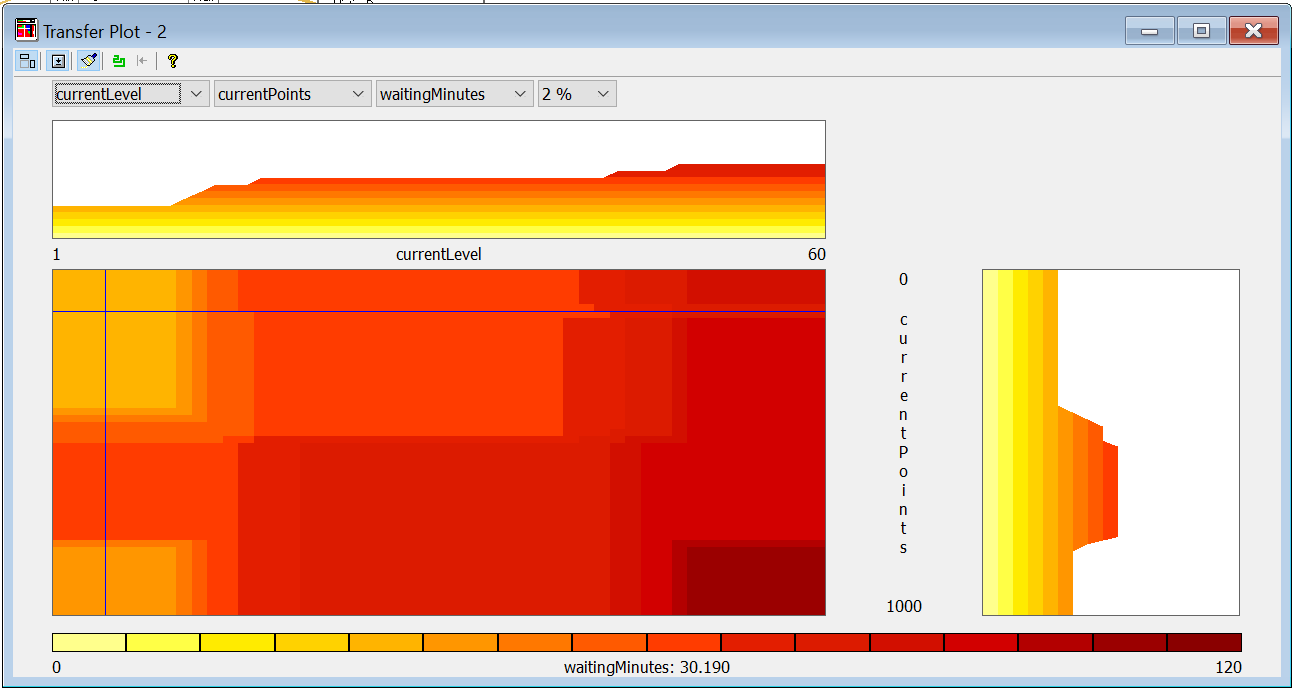
\includegraphics[width=\textwidth]{img/profile1_r12-50}
\caption{Heatmap of \texttt{waitingMinutes} activation for \texttt{R12}=50\%}
\label{fig:prof1_3d50} 
\end{figure}

\begin{figure}[H]
\centering
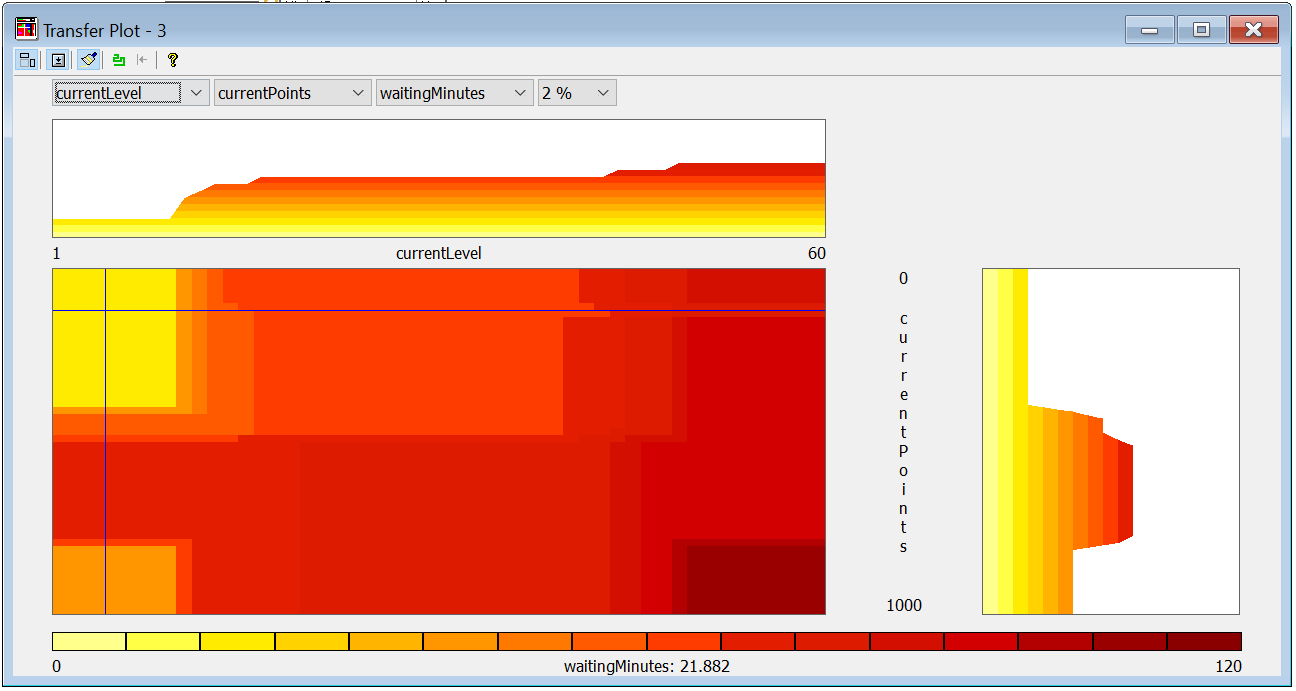
\includegraphics[width=\textwidth]{img/profile1_r12-10}
\caption{Heatmap of \texttt{waitingMinutes} activation for \texttt{R12}=10\%}
\label{fig:prof1_3d10} 
\end{figure}






\section{Problem Analysis}
\label{sec:PA}

To analyze this problem thoroughly, we describe the used predicates (subsection \ref{sub:pred}), the possible initial and goal states (subsection \ref{sub:igs}), the operators (subsection \ref{sub:op}), the search space (subsection \ref{sub:ss}) and special cases (subsection \ref{sub:sc}).

\subsection{Predicates}
\label{sub:pred}

The used predicates are the following:

\begin{itemize}
	\item \texttt{Robot-location(o)}: The robot is in office $ o $. We chose a coordinate based representation of offices where each $ o $ is defined by its coordinates $[x, y]$. 
	\item \texttt{Robot-free}: The robot does not have any coffee loaded.
	\item \texttt{Robot-loaded(n)}: The robot has $ n $ cups of coffee loaded with $n \in \{1, 2, 3\} $.
	\item \texttt{Petition(o, n)}: $ n $ cups of coffee are required in office $ o $ with $n \in \{1, 2, 3\} $.
	\item \texttt{Served(o)}: Office $ o $ has been served.
	\item \texttt{Machine(o, n)}: There is a coffee machine in office $ o $ that produces exactly $ n $ cups of coffee with $n \in \{1, 2, 3\} $.
	\item \texttt{Steps(x)}: The robot has moved $ x $ steps with $ x \in \mathbb{N}_0 $.
\end{itemize}

\subsection{Intitial and Goal States}
\label{sub:igs}

The \textbf{initial state} of any problem is composed as follows: 

\begin{itemize}
	\item \textbf{Required predicates}: \textit{Robot-free}, \textit{Steps(0)}, \textit{Robot-location(o)} where $ o $ is a valid office location.
	\item \textbf{Optional predicates}: One or more \textit{Petition(o,n)} with at most one petition for each office. 
	\item \textbf{Conditionally required predicates}: For each $ n^* \in \{1, 2, 3\} $ that occurs in a $ Petition(o, n^*) $, there has to be at least one \textit{Machine(o, n)} with fitting $ n = n^* $ in order to guarantee that the problem is solvable.
\end{itemize}

The \textbf{final state} of any problem is composed as follows:

\begin{itemize}
	\item \textbf{Optional predicates}: A \textit{Robot-location(o)} can be specified.
	\item \textbf{Conditionally required predicates}: For each $o^*$ that occurs in a $ Petition(o^*, n)$, there must be exactly one $ Served(o^*) $ predicate in the final state.
\end{itemize} 
 

\subsection{Operators}
\label{sub:op}

This problem contains three operators that can be applied to reach the final state starting from the initial state. These operators are: $Move(o_1, o_2)$, $Make(o,n)$ and $Serve(o,n)$.
\subsubsection*{Move:}
The operator \textbf{$Move(o_1, o_2)$} allows the robot to move between offices and is set up in the following way:
\begin{itemize}
	\item \textbf{Preconditions}: Robot-location($o_1$), Steps($x$).
	\item \textbf{Add}: Robot-location($o_2$), Steps($x+distance(o_1, o2)$).
	\item \textbf{Delete}: Robot-location($o_1$), Steps($x$).
\end{itemize}

\subsubsection*{Make:}
The operator \textbf{$Make(o, n)$} allows the robot to make coffee in an office with a machine and is set up in the following way:
\begin{itemize}
	\item \textbf{Preconditions}: Robot-location($o$), Robot-free, Machine($o,n$).
	\item \textbf{Add}: Robot-loaded($n$).
	\item \textbf{Delete}: Robot-free.
\end{itemize}

\subsubsection*{Serve:}
The operator \textbf{$Serve(o, n)$} allows the robot to serve coffee and is set up in the following way:
\begin{itemize}
	\item \textbf{Preconditions}: Robot-location($o$), Robot-loaded($n$), Petition($o,n$).
	\item \textbf{Add}:  Served($o$), Robot-free.
	\item \textbf{Delete}: Robot-loaded($n$), Petition($o,n$).
\end{itemize}

\subsection{Search Space}
\label{sub:ss}

The search space of a problem is the subset of the state space that can be reached by applying the operators, starting at the initial state. The nodes in the search space correspond to states of the world, while the edges correspond to state transitions through operators.

To compute the size of the search space we have to consider how many states we can reach from a given initial state by only applying our operators. In order to compute the size of the search space we take the following considerations into account:

\begin{itemize}
	\item The predicate Robot-location($o$) is always present exactly one time in each state, since it is required in the initial state and no operator adds this predicate without deleting a different instantiation of it and vice versa. There are $36$ different values for $o$ (one for every office in the world. 
	\item Robot-free and Robot-loaded(n) cannot be part of a state at the same time (see Make and Serve operators). Robot-loaded(n) can take three different values: $1, 2$ and $3$. This leads to $4$ different combinations: Robot-free, Robot-loaded($1$), Robot-loaded($2$) and Robot-loaded($3$).
	\item The Petition($o,n$) predicates are taken from the initial state and can then be removed via the Serve operator. Since each Petition predicate can either still be present or replaced with a Served predicate, the number of possible states is $2^{|P|}$ where $|P|$ is the number of petitions in the initial state.
	\item The predicate Steps($x$) is only present once, but $x$ can take a arbitrary integer value larger than 0.
\end{itemize}

The Steps($x$) predicate makes the search space infinitely large. Since our goal is to both reach the final state while minimizing $x$, we will consider the search space ignoring $x$ and then later twist our algorithm in a way to explore the search space with consideration to keeping $x$ small.

Ignoring the Steps($x$) predicate, our search space is of size $36 \cdot 4 \cdot 2^{|P|}$ with $|P|$ being the number of petitions in the initial state. The size of the search space grows exponentially with the number of petitions.


\subsection{Special Cases}
\label{sub:sc}

Some combinations of initial states and final states are not able to be solved. This is the case when the final state is not part of the search space. An example case for this scenario is a Petition($o,n_p$) predicate that does not have a matching Machine($o, n_m$) with $n_p=n_m$. 





\section{Planning Algorithm}
\label{sec:PlaniAlg}


\subsection{STRIPS Algorithm}
The implementation is based on the STRIPS algorithm which works in the following way:

The STRIPS is provided with an initial state, a final state (containing the goals of the problem) and a set of operators. We use a simplified version of STRIPS where the goal state cannot state predicates that need to be false - it can only specify a conjunction of predicates that need to be true in the end.

The STRIPS algorithm uses a stack that can contain single predicates, lists of predicates and operators to calculate a plan of operators that reach the final state starting from the initial state. 

A pseudo-code example of the STRIPS algorithm can be found in listing \ref{code:strips}.

\begin{lstlisting}[language=Java, 
	caption=The STRIPS algorithm, 
	keywordstyle=\color{blue},
	stringstyle=\color{red},
	commentstyle=\color{magenta},
	label = {code:strips}]
State initialState, finalState
State currentState = initialState;
List<Operator> operators;
Stack stack;
List<Operator> plan;

stack.push(finalState.predicateList);
for(predicate : finalState.predicateList):
   stack.push(predicate);

while(!stack.isEmpty()):
   element = stack.pop();
   
   case element instanceof Operator:
      currentState.apply(element);
      plan.add(element);
   
   case element instanceof List<Predicate>:
      for(predicate : element):
         if predicate not true in currentState:
            stack.push(predicate);
   
   case element instanceof Predicate:
      if element.isFullyInstantiated():
         if element not true in currentState:
            operator = findOperatorToResolve(element);
            stack.push(operator);
            stack.push(operator.preconditions);
            for(predicate : operator.preconditions):
               stack.push(predicate);
         else: 
            // Look for constant c to instantiate element.
            // Set c in entire stack.
            instantiate(element);

return plan;
\end{lstlisting}

\subsection{Heuristics}
\label{subsub:heuristics}

In our specific implementation of the STRIPS algorithm to solve the coffee problem, we use two different heuristics to reduce the number of steps $x$ that are needed to achieve the final state. These heuristics determine in which order the predicates belonging to a list of predicates get pushed onto the stack, and which constant is selected out of several options when instantiating the predicates.

\subsubsection{The Served-Heuristic}

The Served-Heuristics determines in which order the robot processes the different petitions to serve the coffee. If the petitions are processed in a random order or simply based on their position in the description of the world, the robot is likely to make a lot of unnecessary steps. The optimal solution here belongs to the class of the Traveling Salesman Problem and is too complex to exactly compute for a large number of petitions.

Computing all possible paths along the petitions in a brute-force way requires $O(2^{|P|})$ steps, which is unfeasible for large numbers of petitions $P$. In our implementation we resorted to the nearest-neighbor heuristic (NN-heuristic) to get a good solution for this problem with relatively little computational effort. The steps of this algorithm are the following:

\begin{enumerate}
	\item Start at the beginning position of the robot.
	\item Find shortest distance between current position and an unvisited Served predicate $S^*$.
	\item Save $S^*$ to sequence and set current position to $S^*$.
	\item Mark $S^*$ as visited.
	\item If all Served predicates are visited, terminate
	\item Go to step 2.
\end{enumerate} 

The difference between visiting petitions in their order (from $P_1$ to $P_4$) or choosing a path based on the NN-heuristic can be seen in figure \ref{fig:1}. While the path based on the petition number requires 21 steps, the NN-heuristic only requires 17 steps. Empirical results of the NN-heuristic can be found in section \ref{sec:results}.

\begin{figure}[!ht]
\centering     %%% not \center
\subfigure[21 steps with petition number order]{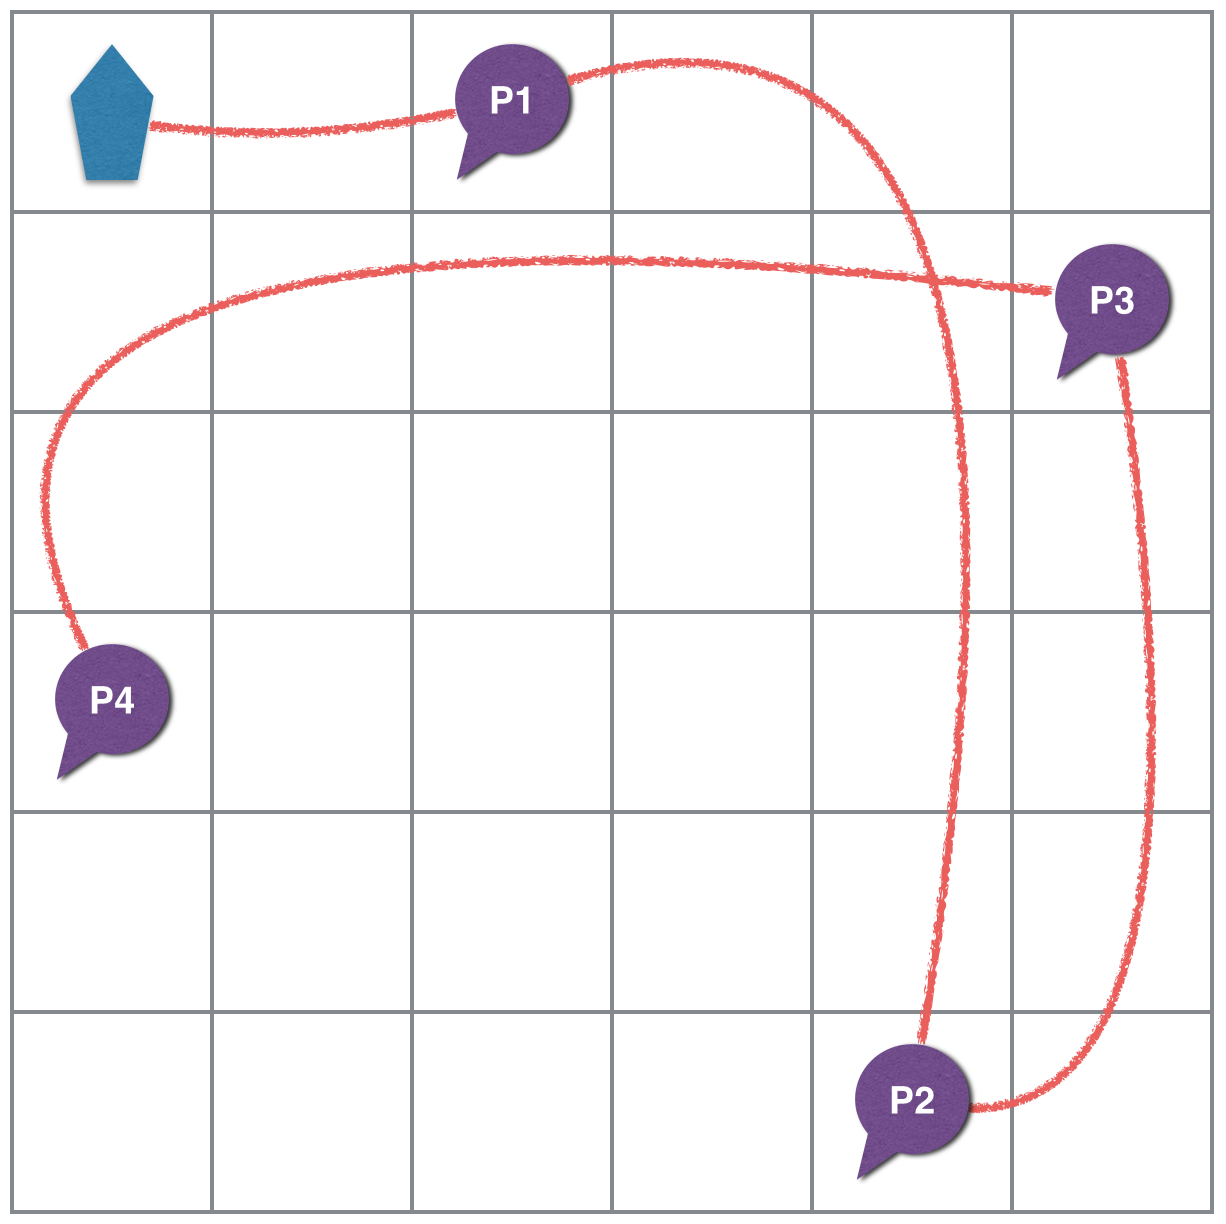
\includegraphics[width=60mm]{img/servedHeur1}}
\subfigure[17 steps with NN-heuristic]{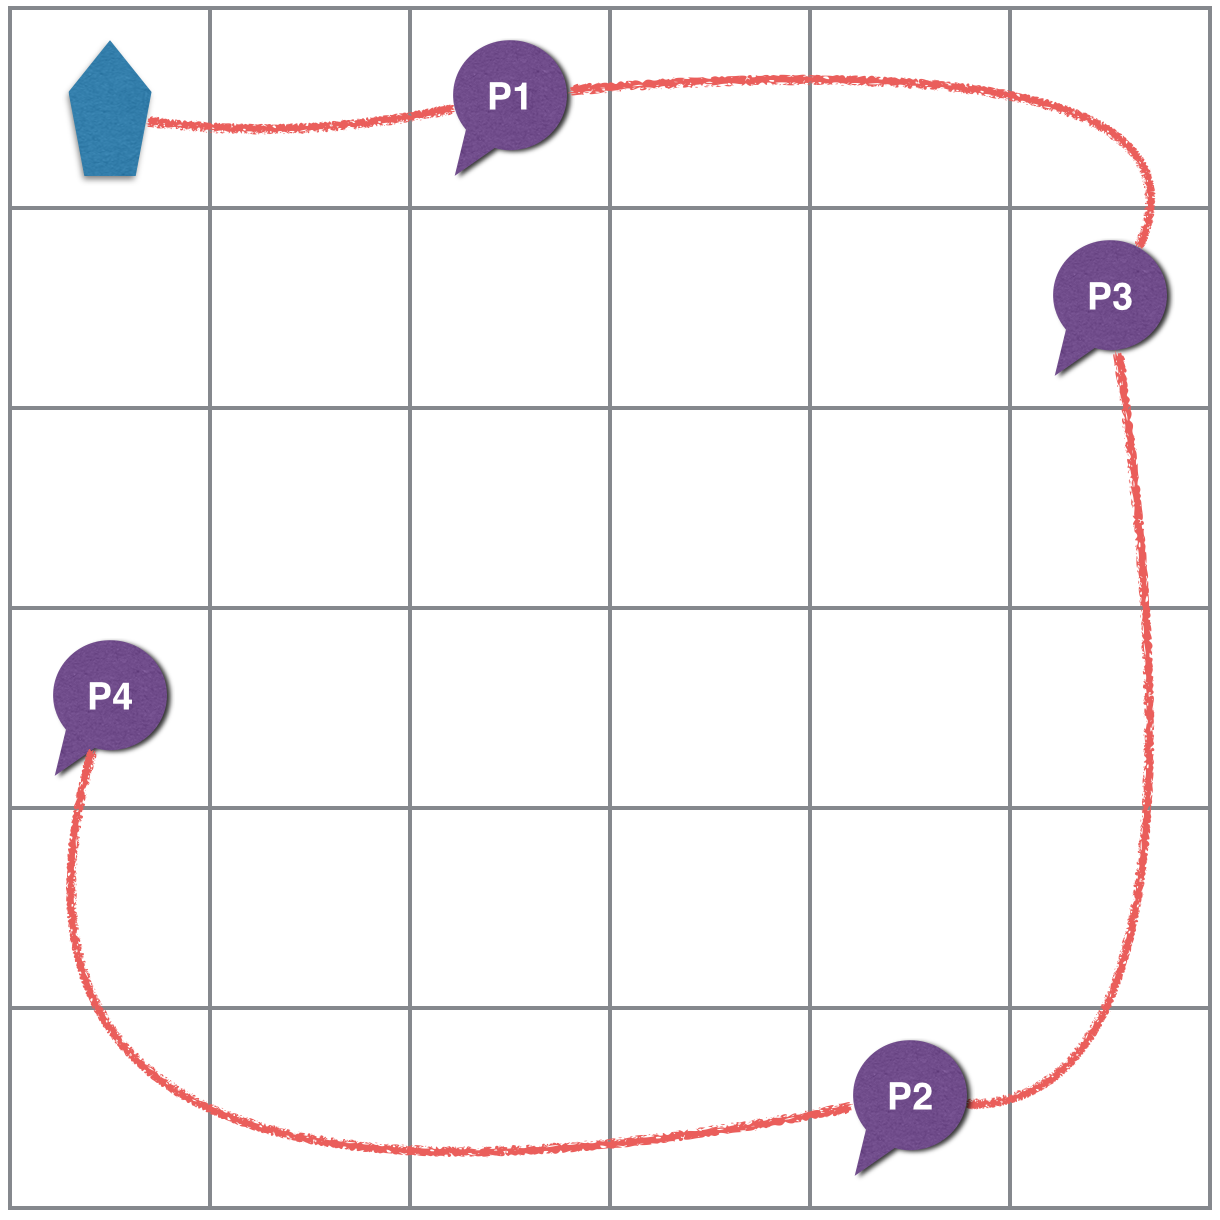
\includegraphics[width=60mm]{img/servedHeur2}}
\caption{Petition Number Order vs. NN-Heuristic}
\label{fig:1}
\end{figure}



\subsubsection{The Machine-Heuristic}

When planning to serve coffee for a specific petition, the planner has to find a suitable machine that can brew the fitting number of cups. In some worlds there might be more than one possible Machine predicate with a fitting $n$. The right choice of machine is focus of our second heuristic.

Without using a heuristic, STRIPS instantiates with an arbitrary compatible machine, which can lead to big detours (as shown in example (a) of figure \ref{fig:2}). A first improvement of the number of steps can be achieved by choosing the machine that is closest to the current position of the robot, as in example (b) of figure \ref{fig:2}. 

In our heuristic we don't only consider the distance between current position and the machine, but also the distance from that machine to the next petition. For the robot position $r$, the machine position $m$ and the petition location $p$, the distance is calculated as:

$heurDist(m)  = dist(r, m) + dist(m, p)$

We then choose the machine $m$ with the smallest $heurDist(m)$.

\begin{figure}[!ht]
\centering     %%% not \center
\subfigure[First machine]{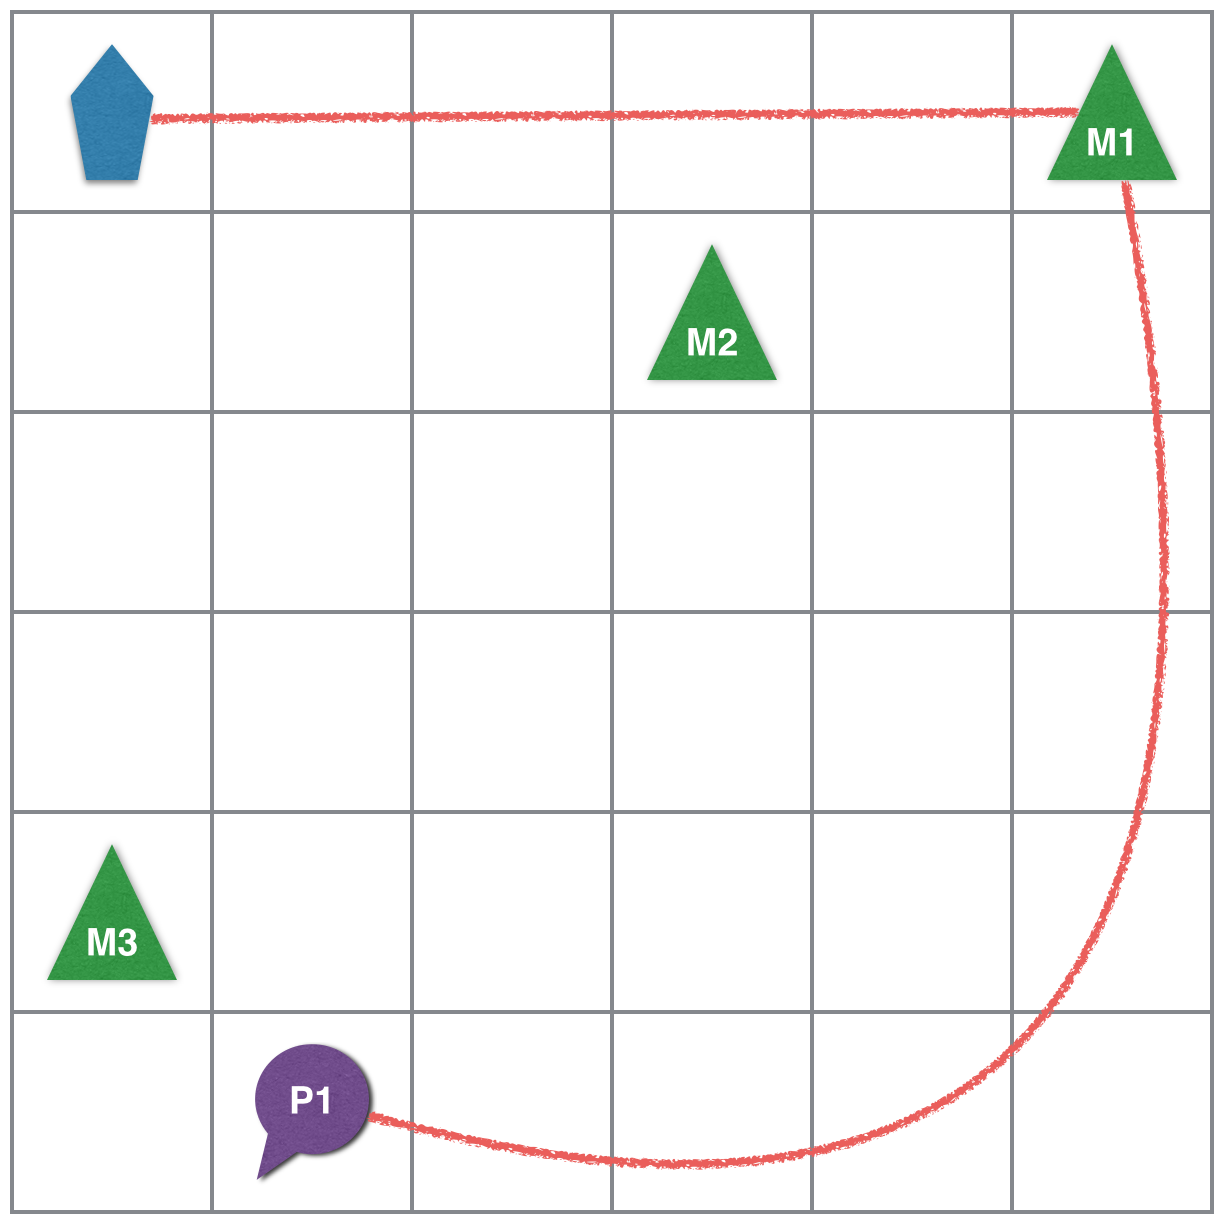
\includegraphics[width=40mm]{img/mHeur1}}
\subfigure[Nearest machine]{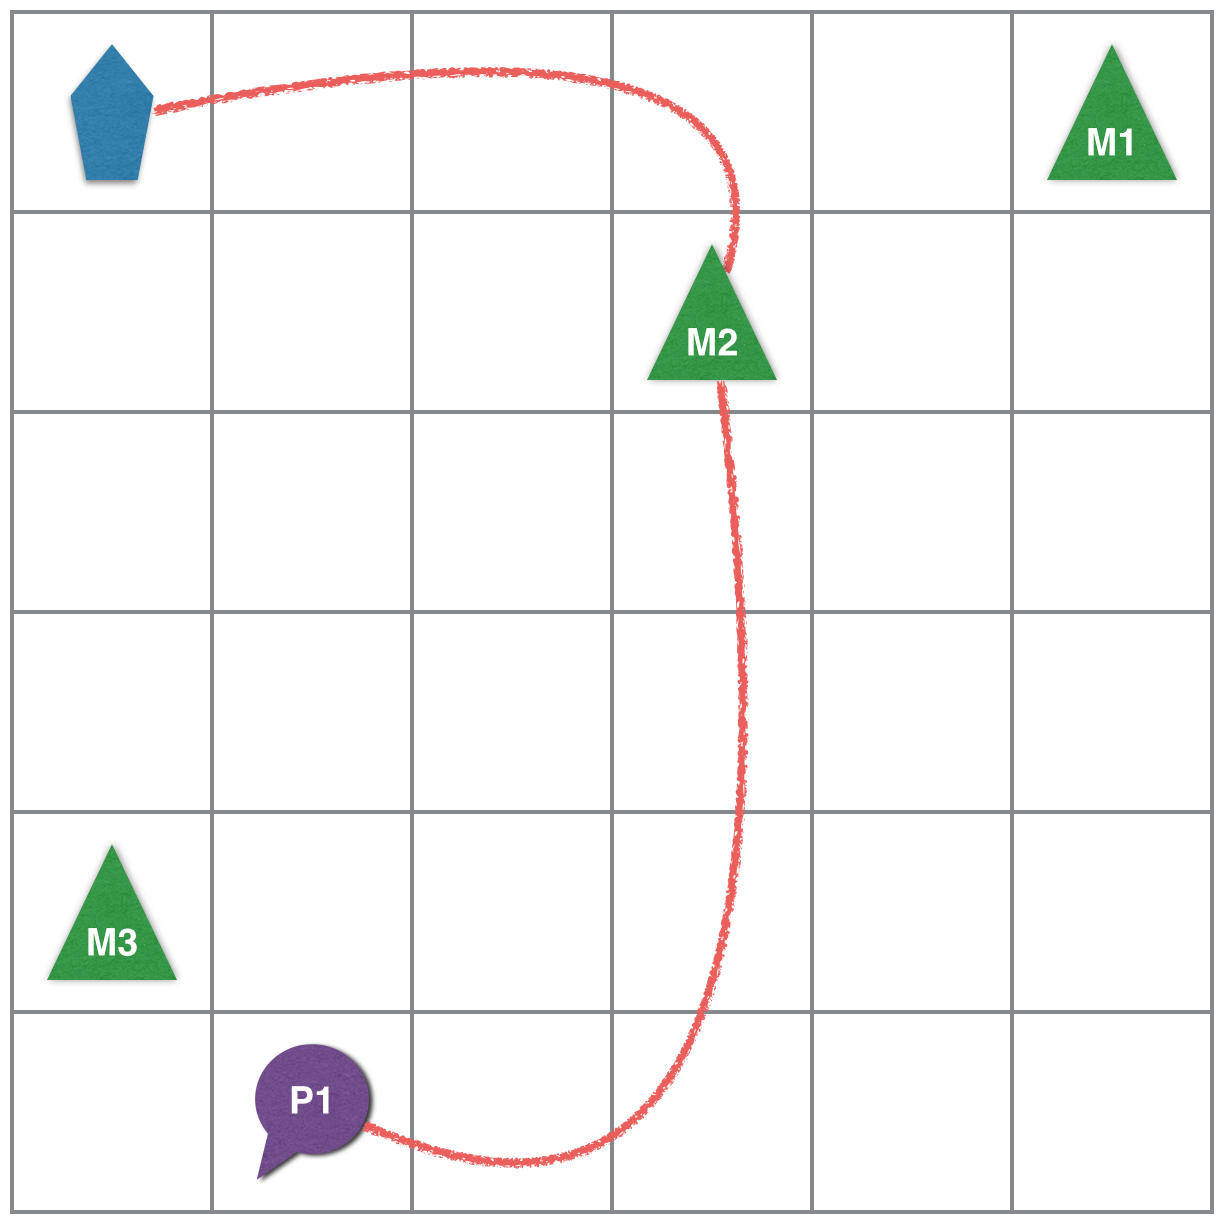
\includegraphics[width=40mm]{img/mHeur2}}
\subfigure[Best total distance]{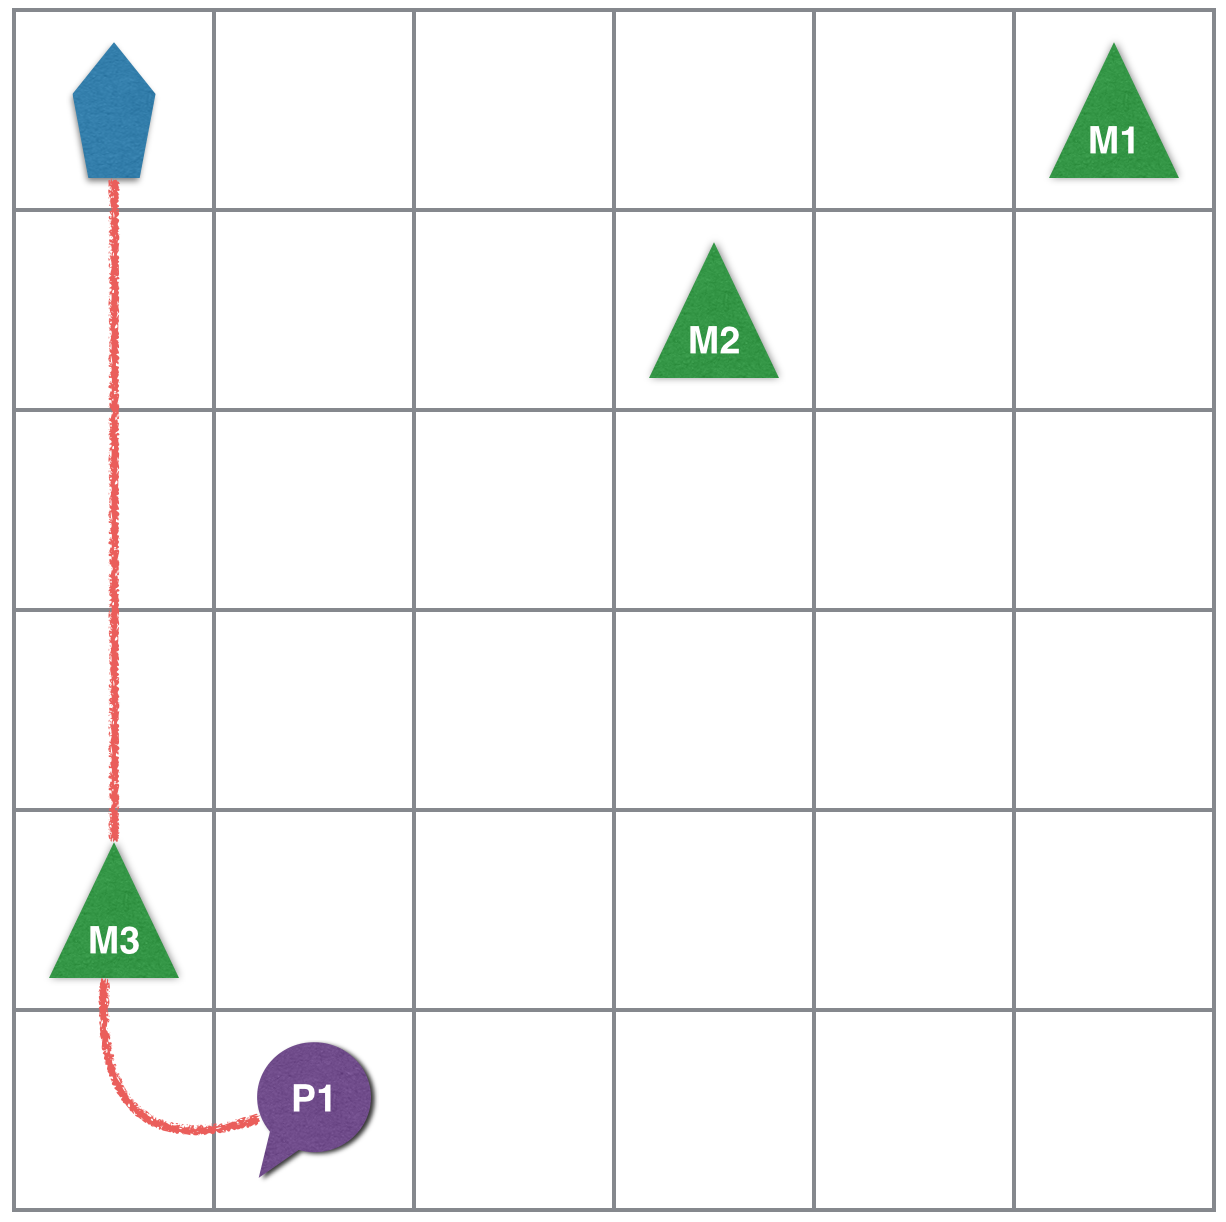
\includegraphics[width=40mm]{img/mHeur3}}
\caption{Comparison of Machine Selection}
\label{fig:2}
\end{figure}

Empirical results of this heuristic can be 


\section{Implementation}

% TODO: general class structure

\subsection{Class structure}

\begin{figure}[hbt]
  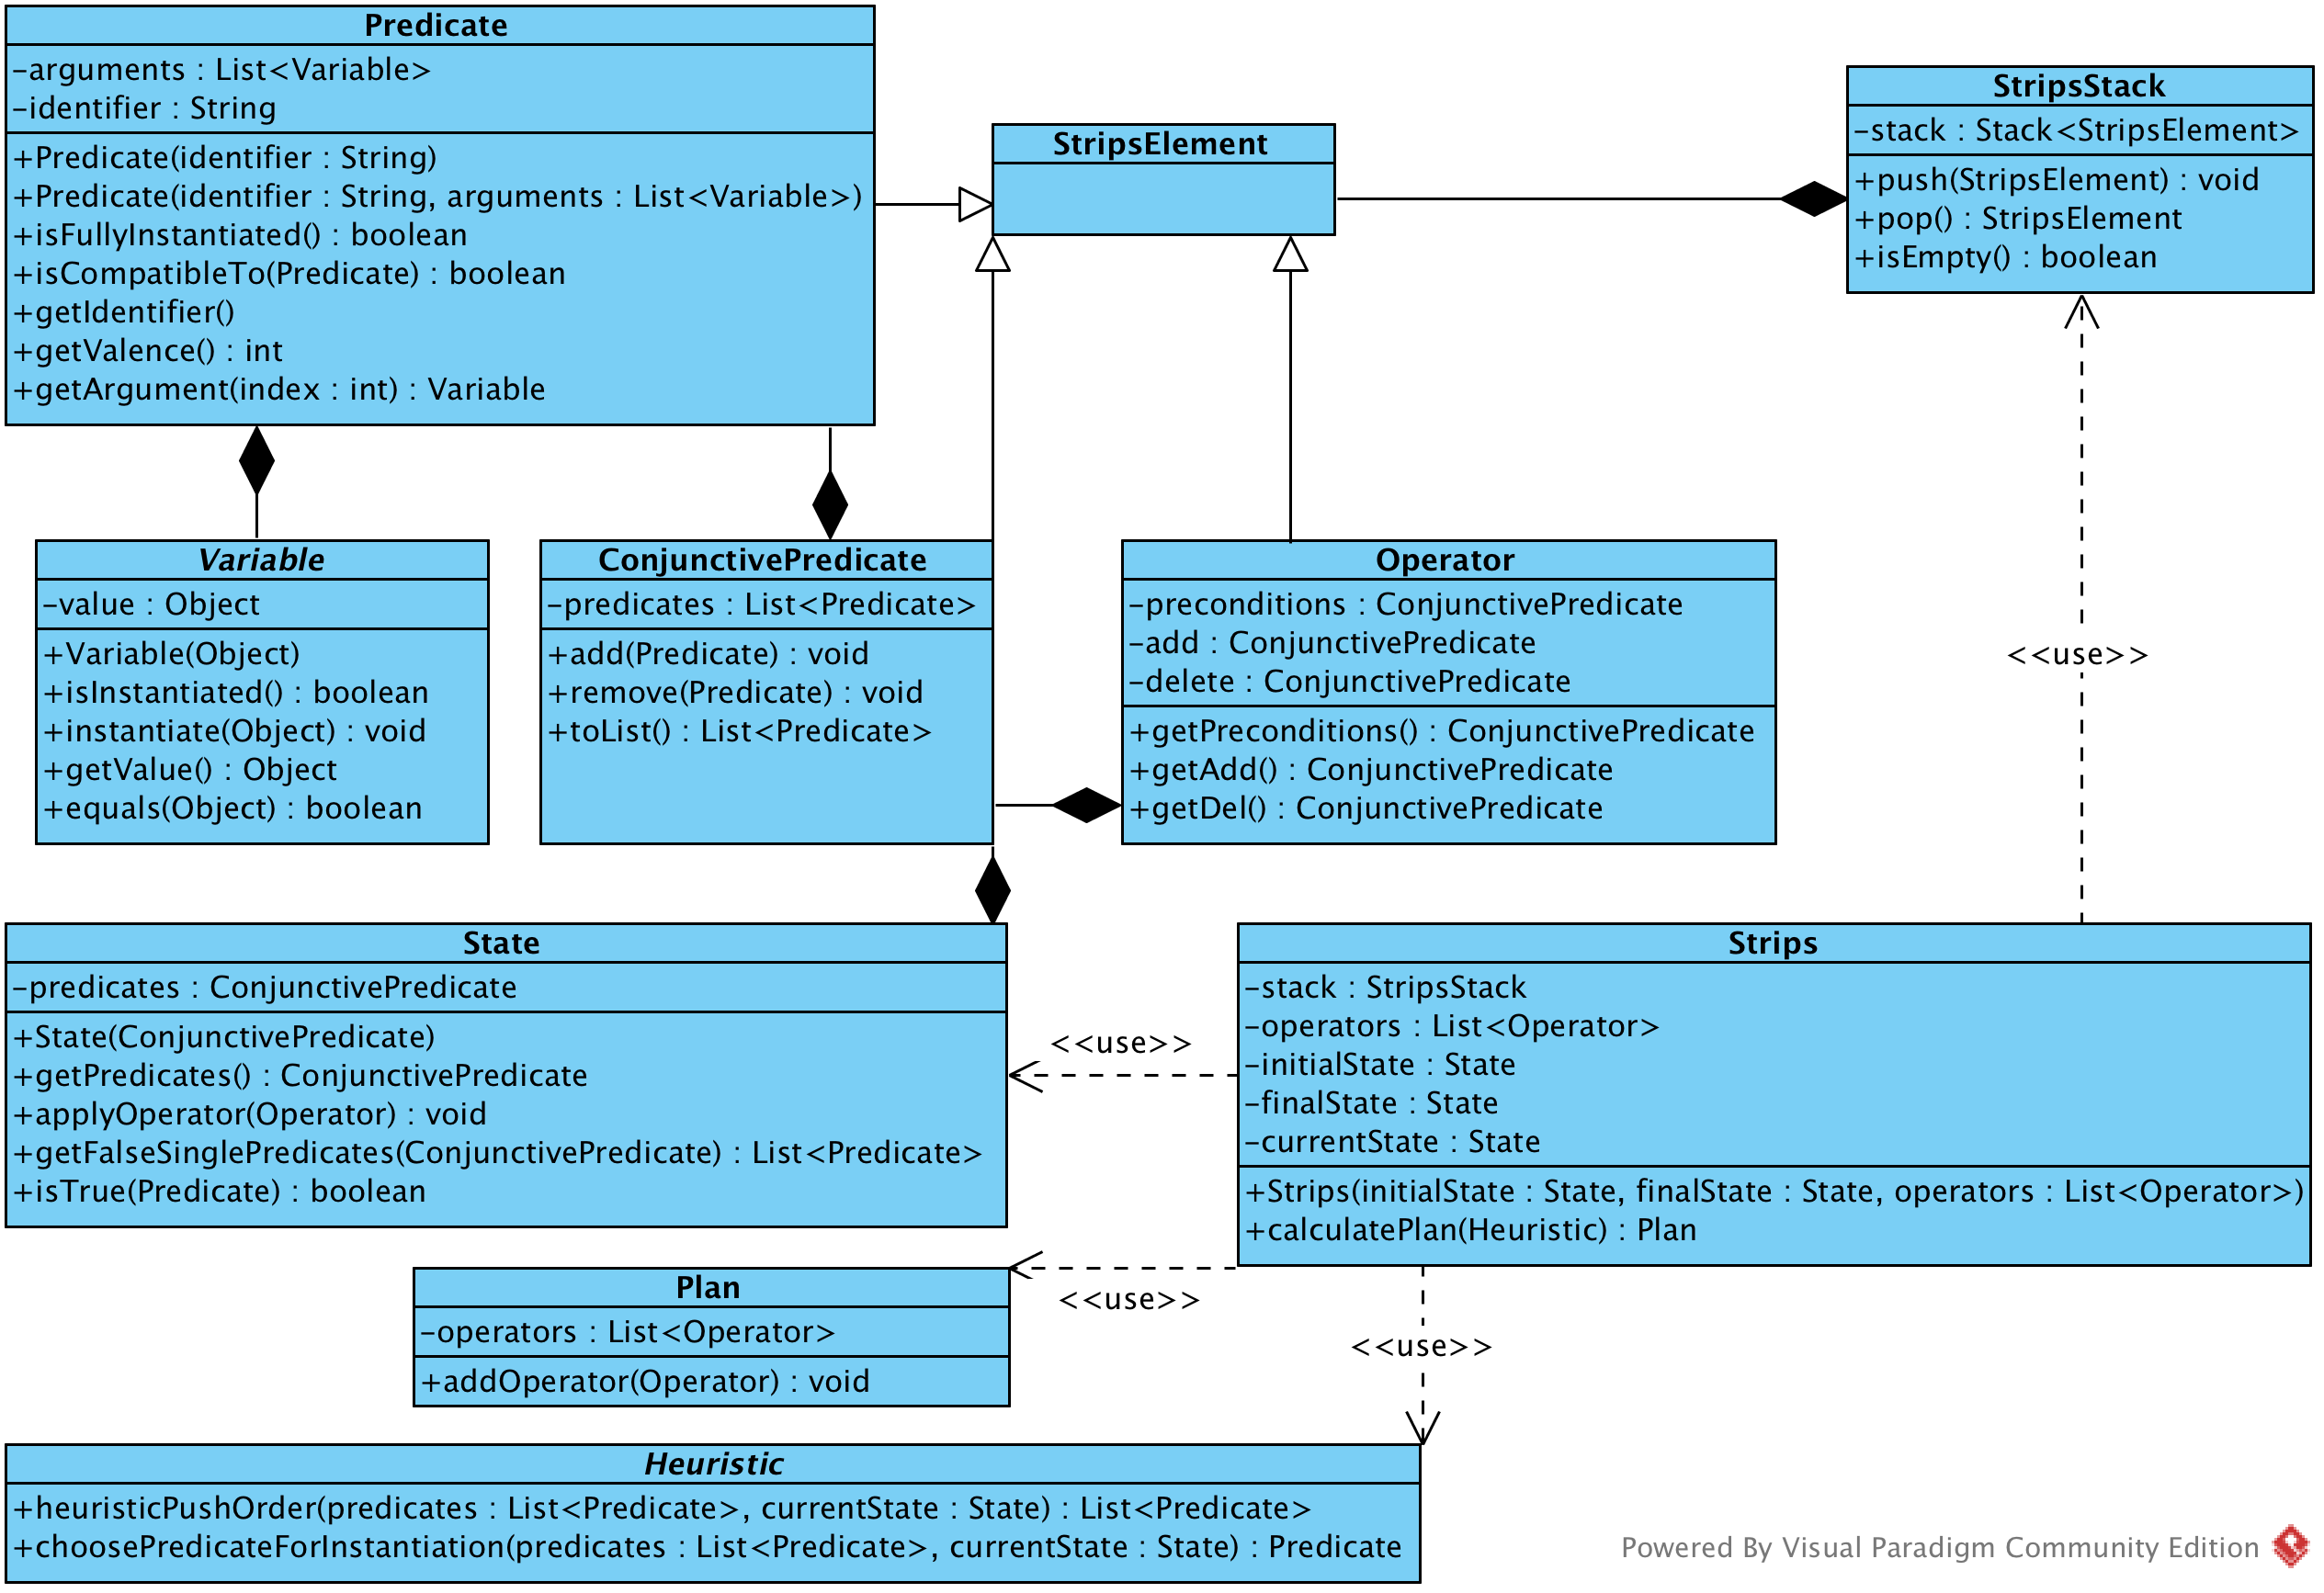
\includegraphics[width=1.1\textwidth]{uml/CD1}
  \caption{UML Class Diagram of STRIPS classes}
\end{figure}

% TODO: specific class strucutre

\subsection{Implementation details}

\begin{lstlisting}[language=Java, caption=Strips method  \textit{instantiate}]
private void instantiate(Predicate singlePred, Heuristic heuristic) {
  List<Predicate> compatiblePredicates = new ArrayList<>();
  for (Predicate currPred : this.currentState.getPredicates().toList()) {
    // find all compatible predicates in current state:
    if (currPred.isCompatibleTo(singlePred)) {
      compatiblePredicates.add(currPred);
    }
  }
  ... 
  // Heuristic chooses one candidate from compatiblePredicates
  Predicate chosenPred = heuristic.choosePredicateForInstantiation(
				compatiblePredicates, currentState);
				
  // instantiate with singlePred with constants of chosenPred
  for (int i = 0; i < chosenPred.getValence(); i++) {
    if (!singlePred.getArgument(i).isInstantiated()) {
      // instantiate updates the java object of the variable.
      // all references to this variable in other predicates
      // will now reference to the instantiated variable.
      singlePred.getArgument(i).instantiate(
                   chosenPred.getArgument(i).getValue());
    }
  } 
}
\end{lstlisting}

\section{Tests}

We designed both manually designed three different worlds with increasing complexity and 1000 random worlds with random complexity.

\subsection{Manually Created Worlds}

The first example \texttt{data/examples/test1} is a simple world with only one Machine and one Petition:

\texttt{InitialState=Robot-location(o1);Machine(o16,1);Petition(o26,1);Robot-free; Steps(0);
GoalState=Robot-location(o7);Served(o26);}

The second example \texttt{data/examples/test2} is a more complex world with now two Machines and one Petition:

\texttt{InitialState=Robot-location(o1);Machine(o16,1);Machine(o14,1);Petition(o26,1); Robot-free; Steps(0);
GoalState=Robot-location(o7);Served(o26);}

The third example \texttt{data/examples/test2} is even more complex  with two Machines and now four Petitions:

\texttt{InitialState=Robot-location(o1);Machine(o29,1);Machine(o8,1);Petition(o3,1); Petition(o32,1);Petition(o18,1);Petition(o19,1);Robot-free; Steps(0); 
GoalState= Robot-location(o7);Served(o3);Served(o32);Served(o18);Served(o19);}


\subsection{Automatically created worlds}

We created 1000 random worlds. Each of these worlds has between 3 and 9 petitions (at least one for each possible $n$) and between 3 and 9 machines (at least one for each possible $n$). The generated examples are attached to this report, see appendix \ref{app:included}.
\section{Results}
\label{sec:results}

\subsection{Manually Created Worlds}

\begin{figure}[!hbt]
  \centering
  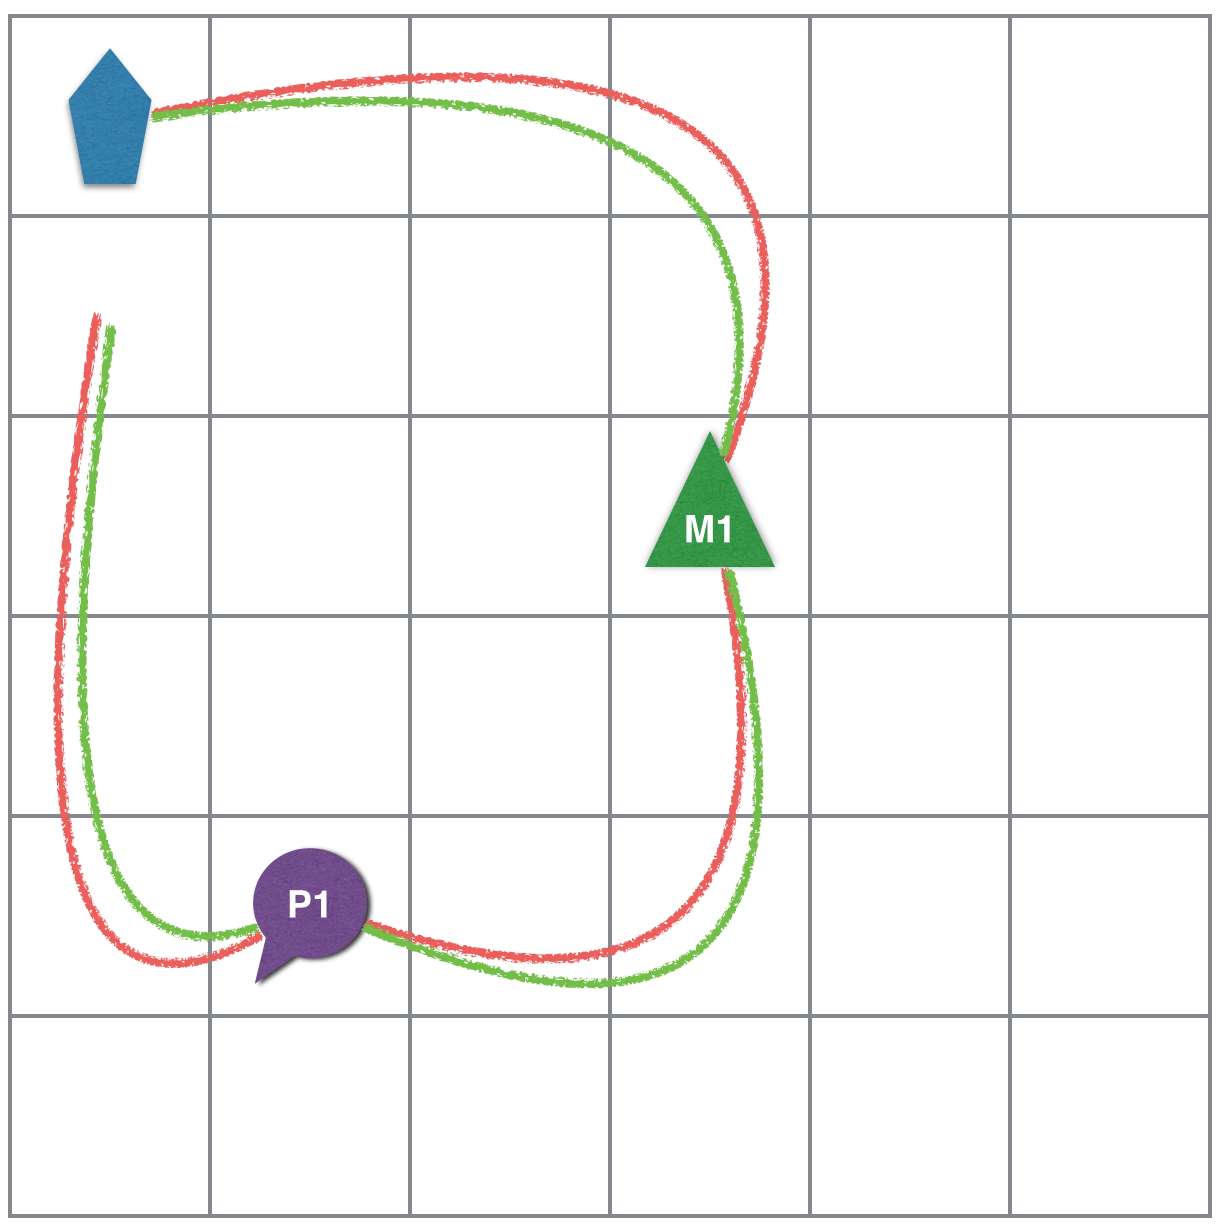
\includegraphics[width=0.5\textwidth]{img/t1}
  \caption{Results for first manually created example}
  \label{fig:t1}
\end{figure}

\begin{figure}[!hbt]
  \centering
  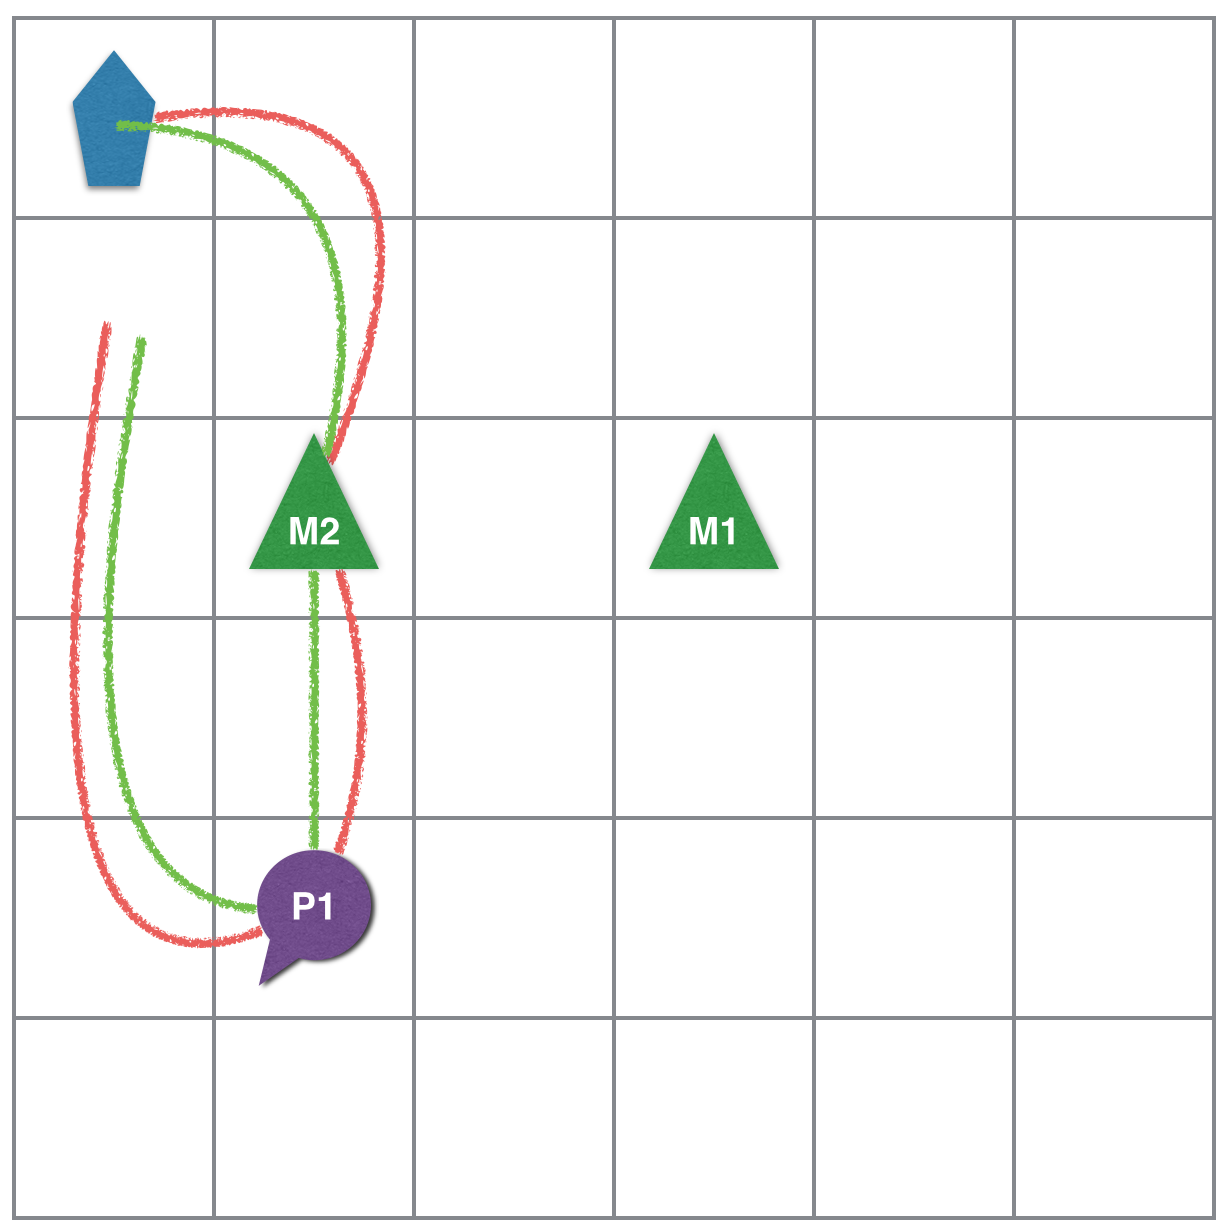
\includegraphics[width=0.5\textwidth]{img/t2}
  \caption{Results for second manually created example}
  \label{fig:t2}
\end{figure}

\begin{figure}[!hbt]
  \centering
  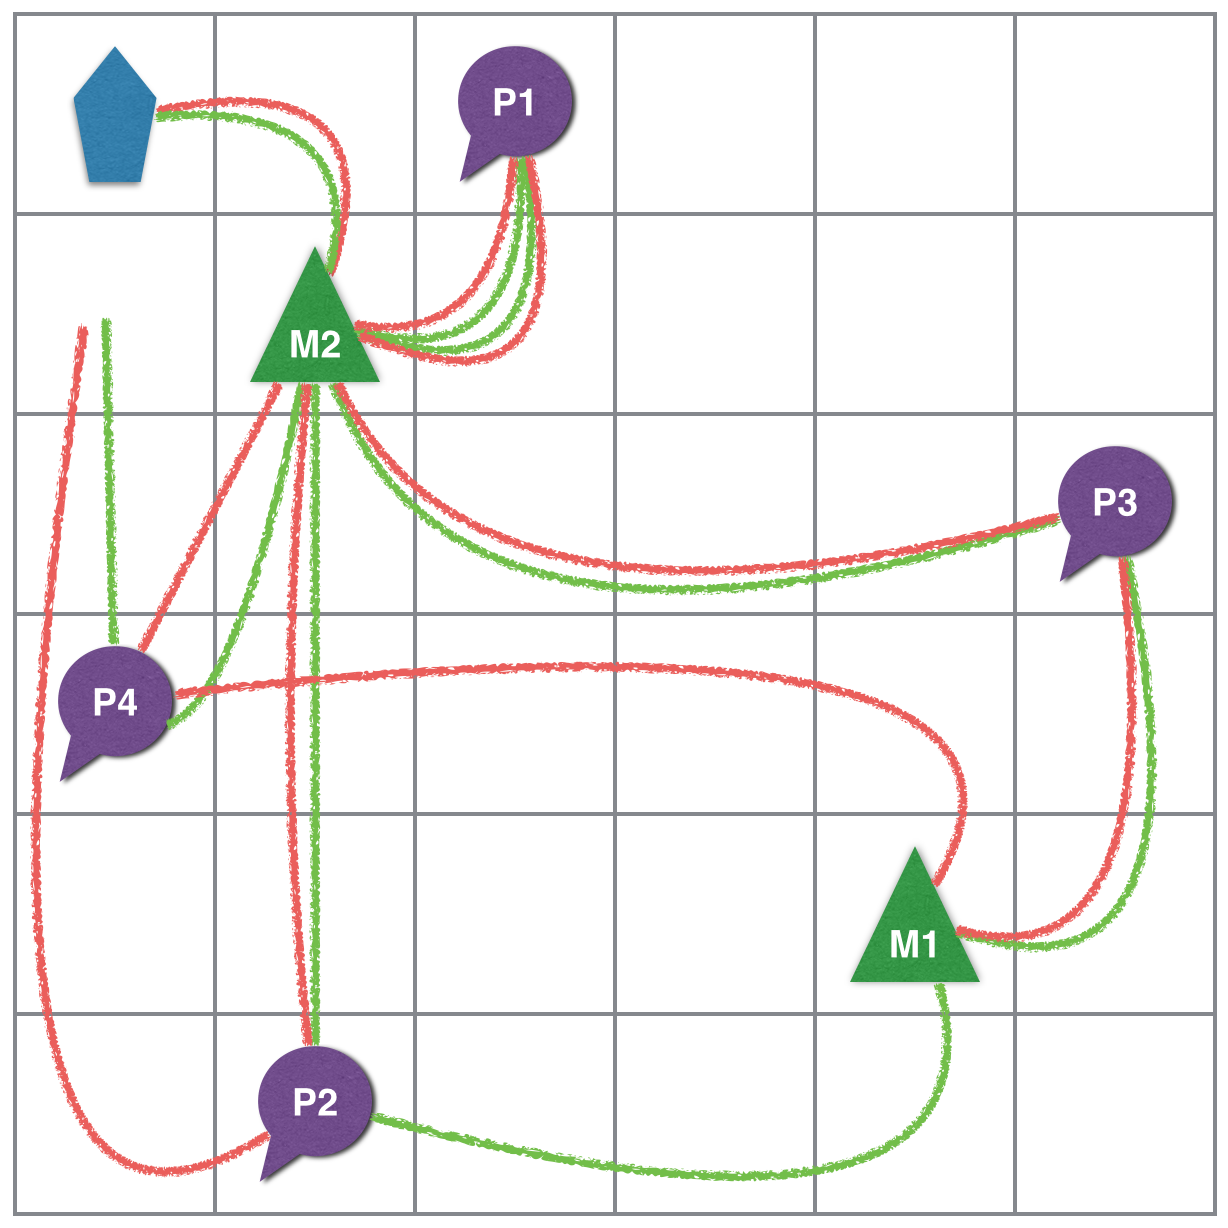
\includegraphics[width=0.5\textwidth]{img/t3}
  \caption{Results for third manually created example}
  \label{fig:t3}
\end{figure}

\subsection{Automatically created worlds}

Figure \ref{fig:abc1} shows the average result (blue dot) and standard deviation (blue bar) of the step error for different heuristics. The step error is defined as the difference between the steps of the optimal solution and the steps that the planner came up with.

NN-TS means, that the NN-heuristic was used to determine the order of petitions. Random means, that a random order of petitions was used. Closest-M means, that the Machine predicate heuristic was used, while First M corresponds to simply picking the first Machine predicate in the list.


\begin{figure}[!hbt]
  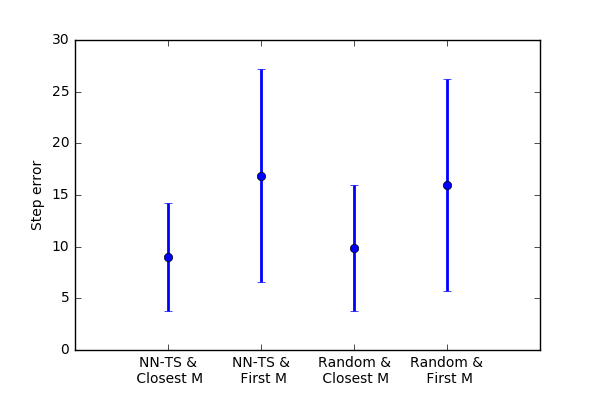
\includegraphics[width=1.1\textwidth]{img/step_error_vs_heuristic}
  \caption{Step Errors for Different Heuristic}
  \label{fig:abc1}
\end{figure}

As we can see in figure \ref{fig:abc1}, using both heuristics yields the best results on average. Not using the NN-heuristics only worsens the results slightly. Deactivating the Machine-heuristic makes the step error increase dramatically - hence it has the highest impact on success.

Figure \ref{fig:abc2} shows how often the different heuristic configuration yielded the smallest step error. Again we can see, that using both heuristics yields the best results with a winner ratio of more than 0.6. The values don't add up to 1.0 because sometimes several strategies had the same result.

\begin{figure}[!hbt]
  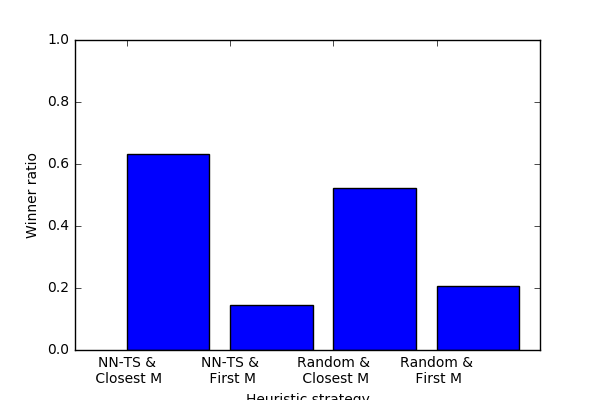
\includegraphics[width=1.1\textwidth]{img/winner_ratio_vs_heuristic}
  \caption{Ratio of Best Solution for Different Heuristic}
  \label{fig:abc2}
\end{figure}

Figure \ref{fig:abc3} shows the relationship between the complexity of the world in terms of numbers of petitions and the average step error. As we can see, for increasing the complexity, using both heuristics yields increasingly better results compared to the other strategies.

\begin{figure}[!hbt]
  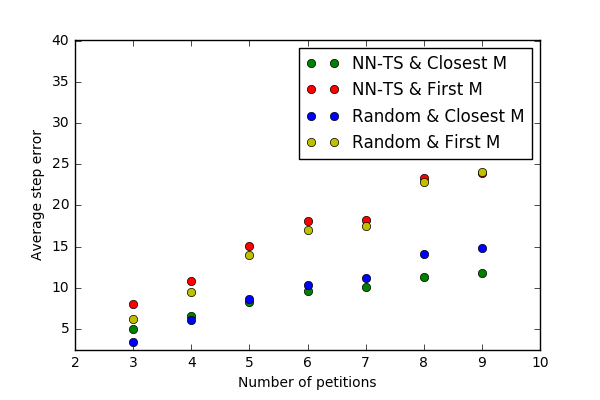
\includegraphics[width=1.1\textwidth]{img/avg_error_vs_petitions}
  \caption{Average Result and Petition Complexity}
  \label{fig:abc3}
\end{figure}

Figure \ref{fig:abc4} shows the relationship between the complexity of the world in terms of numbers of machines and the average step error. There is less correlation between machine complexity and the step error, than we observed with the petition complexity.

\begin{figure}[!hbt]
  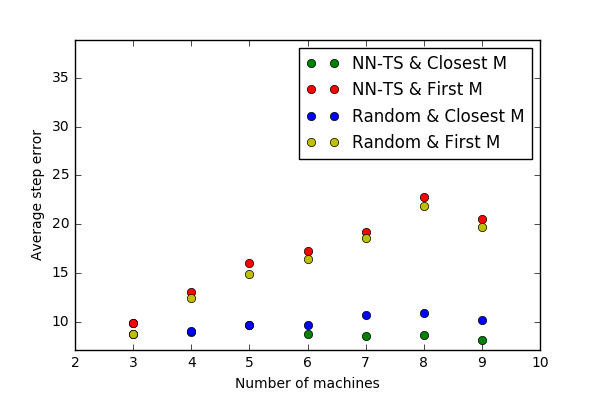
\includegraphics[width=1.1\textwidth]{img/avg_error_vs_machines}
  \caption{Average Result and Machine Complexity}
  \label{fig:abc4}
\end{figure}


\section{Outlook}

Better algorithm than NN to get a good round trip of petitions

Test on larger fields. Some first experiments on worlds with a size of 100,000 fields with several ten-thousands of petitions have shown that the two used heuristics managed to reduce the number of steps from about 4 million to about 20,000 while only requiring approximately 15\% more computation time. The optimal solution could not be computed with brute force in this case since the sheer number of possible permutations exceeds available computation power by far.



\clearpage
\begin{appendices}
\section{Included Files}
\label{app:included}

The project containing this report contains the following directories:

\begin{itemize}
	\item \textbf{/bin} contains the \texttt{.class} files of the project
	\item \textbf{/data}:
	\begin{itemize}
		\item \textbf{/examples} contains the manually created examples test1, test2, test3. It also contains the example given in the task description as test0.
		\item \textbf{/generated} contains the data we generated for our experiment. To repeat the experiment, follow the instructions in the next section of the appendix.
		\item \textbf{/out} contains the output of \texttt{Solve.main} when running the problem solver on a new file. Consider the instructions in the next section of the appendix.
	\end{itemize}
	\item \textbf{/report}
	\begin{itemize}
		\item \textbf{report.pdf} is this report
		\item \textbf{/img} contains the figure used in the report
		\item \textbf{/uml} contains the UML class diagrams used in this report.
	\end{itemize}
	\item \textbf{/src} contains the source code of this project.
\end{itemize} 


\section{Eclipse Instructions}


\begin{enumerate}
	\item Import the project via \texttt{File > Import > Existing Projects into Workspace}
	\item Navigate to class \texttt{problem.Solve}
	\item Choose the input file for the main method by either:
	\begin{itemize}
		\item Changing the constant \texttt{INPUT\_PATH} to the desired path, or
		\item Going to \texttt{Run > Run Configuration > Arguments > Program arguments} and copying the relative or absolute file path in the first line.
	\end{itemize}
	\item Run the main method of \texttt{problem.Solve}.
	\item The results can be found in the directory \texttt{data/out}.
\end{enumerate}


To run the experiment that our results are based on:

\begin{enumerate}
	\item Navigate to class \texttt{problem.coffee.validator.CoffeeExperiments}.
	\item Run the main method.
	\item Results can be found in the directory \texttt{data/generated}:
	\begin{itemize}
		\item \texttt{steps...} contains the number of steps for the different methods.
		\item \texttt{test...}
		\item test\_matrix
	\end{itemize}
	
\end{enumerate}


\end{appendices}

\end{document}
